This chapter presents the empirical work that this thesis turns on:
the cliff sweep on which H1, H2, and the compounding-error model are
based; the model-scaling sweep whose result is reported as
Corollary~1; the frontier validation that promotes the
model-independence claim from small-model evidence to a
cross-architecture result inside a defined calibrated regime; the
retrieval-augmented-generation pipeline catalogue (H3); the
summary-level inference-disclosure measurement (H4); and the
information-density scaling result on real benchmarks reported as
Corollary~2. The chapter is organised around the falsifiable claims
rather than the chronology of the runs; canonical results directories
under \texttt{results/} are referenced for each section so that
every number is traceable to an immutable artefact on disk.

\section{Pre-specification and Refinement}
\label{sec:prereg_refinement}

The six investigations of this chapter were pre-specified with
falsifiable criteria in \texttt{configs/experiments/h\{1-6\}.yaml}
and \texttt{plan-v3.md}. The six hypotheses and the statistical
protocol were committed to the project repository on 2026-05-21,
prior to the data-generation runs that produced the headline
numbers reported in this chapter (the final sweeps ran from
2026-05-26 onward). This is a pre-specified protocol committed to
version control, not a third-party-frozen pre-registration
(e.g.\ OSF or AsPredicted). The criteria for H3, H5, and H6 were
refined after the sweeps; the refinements are documented as ADR-006--008
in the project repository. The three-tier structure used in the rest
of the chapter is as follows.

\textbf{Three hold as pre-specified.} H1 (workload-level
source-retention F1 does not transferably predict coordination
success), H2 (a sharp cliff
at \mbox{$\ge\!30$\%} drop with $p<0.05$ on \mbox{$\ge\!7/9$} cells),
and H4 (compression reduces inference disclosure with baseline above
priors).

\textbf{Two sharpened.} H5's monotonicity prediction resolved into
the invariance result \textbf{Corollary~1 (Ceiling--Cliff
Separation)}, Section~\ref{sec:corollary1}: $\tau^{*}$ is determined
by the compressor and the task within a calibrated regime, while
planner scale moves the ceiling $p_0$. H6's transfer prediction
resolved into \textbf{Corollary~2 (Information-Density Scaling)},
Section~\ref{sec:corollary2}: the cliff position varies with task
information density $\theta_\text{info}$.

\textbf{One narrowed.} H3's regime sign-flip predicate
($\ge\!5$~pp F1 effect with opposite sign across storage- and
accuracy-bounded regimes) is not satisfied; compress-first dominates
on the tested stack in both regimes (Section~\ref{sec:h3}).

\subsection{Falsifiability criteria as practitioner-relevant minima}
\label{sec:prereg_criteria_defense}

Each numerical bar above ($\rho<0.6$ for H1, $\ge 30\%$ drop for H2,
$\pm 5$~pp F1 sign-flip for H3, paired-bootstrap $p<0.05$ for H4,
$\pm 20\%$ TOST band for Corollary~1, $\Delta\theta_\text{info}
\ge 0.1$ for Corollary~2) was chosen as the smallest effect a
practitioner relying on this thesis would care about, not as an
arbitrary statistical threshold. The catalogue below makes the
rationale for each bar explicit; tool and grid choices (the
ratio grid, the bootstrap budget, the $\theta_q$-at-$0.5 \cdot p_0$
rule) live in \charef{implementation}~Section~\ref{sec:design_choices},
and metric choices in Section~\ref{sec:metric_choices} of this
chapter.

\begin{description}\setlength\itemsep{2pt}
\item[H1 ($\rho < 0.6$, workload-level).] Cohen's convention for
``less than moderate'' rank correlation. A compressor ranking with
$\rho \ge 0.6$ would remain operationally useful to a practitioner
who needs to deploy compression; clearing $\rho < 0.6$ from above
is the bar at which the predictive utility of the single-agent
F1 metric collapses. The verdict's reliance on the workload-level CI
(rather than the pooled CI) follows the unit decision in
Section~\ref{sec:metric_unit}.
\item[H2 ($\ge 30\%$ relative drop, Holm-corrected $p < 0.05$).]
$30\%$ is the smallest coordination-success drop a practitioner
cares about. A $10\%$ drop sits within typical run-to-run variance
on the families this thesis evaluates; a $50\%$ drop is obvious
without measurement; $30\%$ is the value below which the operating
point would still be deployable and above which it would not. The
Holm correction is applied within the $12$-cell family of
(compressor, family) pairs, not across hypotheses, because the H2
claim is internal to that family.
\item[H3 ($\ge 5$~pp F1 effect with opposite sign across regimes).]
$5$~pp F1 is the smallest gap the practitioner cost-model
(EUR-per-workflow, Section~\ref{sec:h3}) makes operationally
meaningful; opposite sign is what would justify regime-conditional
deployment of P1 versus P2 at all. The pre-specified predicate is
what the data did not support, which is the H3 narrative.
\item[H4 (paired-bootstrap $p < 0.05$, positive direction).]
Paired bootstrap because the same workloads appear in the
priors / baseline / compressed conditions; $p < 0.05$ is
conventional; the positive direction is the privacy direction
(compression must reduce, not increase, disclosure). The
construct-validity caveat in Section~\ref{sec:h4_construct} is
about the privacy \emph{interpretation} of a positive effect, not
about whether the effect itself is detectable.
\item[Corollary~1 ($\pm 20\%$ TOST equivalence band).]
The $\pm 20\%$ band is the strict cliff-position-detectability
tolerance reported alongside the $\pm 50\%$ permissive default in
\texttt{validate\_model\_independence}. The permissive band
absorbs the noise inherent in the local-model arm (small samples,
high run-to-run variance); the strict bar is the one a
deployment-grade ``no shift detected'' claim ought to clear, and
is the one the frontier-validation evidence is tested against. The two are
reported alongside each other in
Section~\ref{sec:corollary1}, and the strict bar is what
the on-disk record \texttt{model\_independence\_20pct.json}
quantifies.
\item[Corollary~2 ($\Delta\theta_\text{info} \ge 0.1$ between
dense and distributed benchmarks).]
$0.1$ is the smallest information-density gap that produces a
qualitatively distinct cliff shape on the three benchmarks
evaluated --- below this gap the cliffs are visually
indistinguishable on the AUC-based $\theta_\text{info}$ axis. The
bar is conservative against estimator noise: the empirical gaps in
Table~\ref{tab:corollary2} ($0.48$ between C1 family-a and
MultiHop-RAG, $0.59$ between C1 family-a and HotpotQA) clear it by
several multiples, so the corollary verdict does not turn on the
precise location of the bar within the noise floor.
\end{description}

The motivation for surfacing these defences here is that an
external reviewer will reasonably ask why a particular threshold
was chosen; each one is defensible as a practitioner-relevant
minimum, not an arbitrary statistical choice.

The consolidated table is Table~\ref{tab:verdict_summary}
(Section~\ref{sec:verdict_summary}).

\section{Experimental Protocol}
\label{sec:protocol}

\subsection{The cliff sweep}

The cliff sweep underlies H1, H2, and the calibration step of the
compounding-error model. Four compressors --- LLMLingua-2,
Phi-3-Mini extractive, the instruction-aware filter, and a
truncation baseline --- are evaluated at ten compression ratios
$\{1, 2, 3, 4, 5, 6, 8, 10, 12, 16\}\times$ on the $150$ C1
workloads across the three families. Five seeds per cell give a
total of approximately $30{,}000$ evaluation cells per run. The
canonical results directory is
\texttt{results/h1\_h2\_v2/}; the earlier
three-compressor variant \texttt{results/h1\_h2\_final/} is retained
on disk for backwards-compatibility checks but is not the source of
the headline numbers below. The truncation baseline is the
lower-bound argument: any compressor that does not beat truncation
on the coordination metric is paying training or inference cost for
no coordination-quality return.

Every cell records the coordination-success binary, the
source-retention F1 (token-overlap F1 between the compressed
fragments and the original source text --- the \texttt{qa\_f1}
column H1 analyses, \emph{not} answer-level QA-F1 against a gold
answer), the achieved compression ratio, the
generic token-recall, and the critical-token-recall described in
Section~\ref{sec:ctr} of \charef{implementation}. The
compression cache (Section~\ref{sec:cache}) guarantees that every cell
sees the exact same compressed text for a given (compressor, ratio,
workload) tuple, so within-cell variance is exclusively
planner-side variance, not compressor stochasticity.

\subsection{Statistical protocol}
\label{sec:stats}

The statistical protocol is fixed in advance for every hypothesis.
Effect-size summaries are computed at the workload level, never
the cell level: per-workload means are computed first, and the
$95\%$ bootstrap confidence intervals are constructed by resampling
workloads with replacement~\cite{efron1993bootstrap}, never by
resampling individual seed--cell pairs. The bootstrap method is the
bias-corrected and accelerated (BCa) interval (per the construction in~\cite{efron1993bootstrap})
with $n_\text{boot} = 10{,}000$ resamples on the main H1/H2/H3/H4
verdict pipelines (the per-method defaults of
\texttt{spearman\_with\_ci}, \texttt{paired\_bootstrap\_diff}, and
\texttt{paired\_bootstrap} in \texttt{src/m6/}). The $\theta_q$
resampling pipeline of Section~\ref{sec:cem_match} and the
frontier-$\tau^{*}$ bootstrap of Section~\ref{sec:frontier} run at
$n_\text{boot} = 500$ instead, because both involve repeated curve
fits whose per-iteration cost is substantially higher than a
single-statistic resample. The two-cell comparison
test is the paired Wilcoxon signed-rank
test~\cite{wilcoxon1945}, chosen over the Mann--Whitney $U$
test~\cite{mannwhitney1947} because the same workloads appear in
both conditions, which violates the independence assumption of the
two-sample test. Multiple-comparisons correction is Holm's
sequentially-rejective procedure~\cite{holm1979bonferroni} applied
\emph{within each hypothesis's family}: the $12$ (compressor,
family) cells of the cliff sweep are Holm-corrected jointly for H2;
the three condition pairs of H4 are Holm-corrected jointly for the
disclosure signal and again jointly for the disclosure reduction;
the three pipelines of H3 are Holm-corrected jointly per regime.
Family sizes are deliberately kept narrow because the hypotheses
are independent claims and joint correction across them would be
over-conservative.

The H1 verdict statistic is the \emph{workload-level} Spearman
correlation ($n = 150$ workloads, one mean $\Delta$-pair per
workload, for every compressor; Phi-3-Mini extractive's
$\sim 2.5\times$ achievable-compression ceiling collapses the
upper ratio range and therefore reduces its \emph{pooled} $n$
from $150 \times 9 = 1350$ to $150 \times 5 = 750$, but does not
reduce the workload-level $n$, Section~\ref{sec:phi3}). A pooled
correlation over $n = 150 \times 9$ (workload, ratio) measurements
would over-state significance by roughly an order of magnitude,
because the nine per-workload ratios are repeated measures rather
than independent draws; that pooled $n$ and its asymptotic
$p$-value are therefore retained in Table~\ref{tab:h1_rho} only
as a non-inferential comparison column. The two-tailed asymptotic
$p$ for $H_0: \rho = 0$ is reported at the workload level; the
verdict rests on the BCa bootstrap CI (over workloads) excluding
$0.6$.

Cliff position $\tau^{*}$ is extracted by fitting both a piecewise-%
linear model and a logistic
\[
  f(r) = p_0 + \frac{p_\infty - p_0}{1 + e^{-k(r - \tau^{*})}}
\]
to each cell's coordination-success-versus-ratio curve and selecting
the model with the lower root-mean-squared error. The piecewise fit
is constrained to an interior $10\%$ margin from the sweep
boundaries. This prevents the optimiser from parking $\tau^{*}$ at
$r_{\max}=16$, a degenerate fit the unconstrained optimiser would
otherwise select. $95\%$~bootstrap CIs on $\tau^{*}$ are computed by
resampling the underlying workload means before the curve fit.

\section{Choice of Evaluation Metrics}
\label{sec:metric_choices}

Every metric reported in this chapter is a choice: a different
metric --- in some cases a more conventional one --- would have
produced a different verdict. This section catalogues all metrics
used in the chapter, names the alternative considered and the
reason it was declined, and consolidates the workload-level versus
cell-level statistical-unit decision that the H1 verdict in
particular turns on. The justification for each individual
hypothesis's falsifiability bar (the $\rho < 0.6$ bar for H1, the
$\ge 30\%$ drop for H2, etc.) is in
Section~\ref{sec:prereg_refinement}; this section is about the
choice of metrics themselves, not the cutoffs. Tool-side and
sweep-grid choices --- the ratio grid, the bootstrap budget, the
P3 routing thresholds --- live in
\charef{implementation}~Section~\ref{sec:design_choices}.

\subsection{Catalogue of metrics}
\label{sec:metric_catalogue}

Table~\ref{tab:metric_choices} enumerates the metrics by the point
at which they enter the verdict pipeline. The chapter's verdict
block in each section
($\!$Sections~\ref{sec:h1}--\ref{sec:corollary2}) rests on the
metrics in this table.

{\small
\begin{longtable}{p{3.0cm}p{5.4cm}p{5.4cm}}
\caption{Choice of evaluation metrics. ``Why chosen'' captures the
property each metric measures; ``Alternative declined'' names the
closest competitor and the reason it was not used.}
\label{tab:metric_choices} \\
\hline
Metric & Why chosen & Alternative declined \\
\hline
\endfirsthead
\hline
Metric & Why chosen & Alternative declined \\
\hline
\endhead
\hline
\multicolumn{3}{r}{\textit{(continued on next page)}} \\
\endfoot
\hline
\endlastfoot
\multicolumn{3}{l}{\textit{Task-level outcomes.}} \\
Coordination success (binary per-instance)
  & Directly answers ``did the planner recover the correct answer?'';
    matches the practitioner's deployment question and operationalised
    once in \charef{introduction}~Section~\ref{sec:multi_fragment}.
  & Graded success: the A3 probe (Section~\ref{sec:a3_probe}) shows
    binary is justified on dense tasks; the graded refinement is
    named as future work on distributed tasks. \\
Token-overlap F1 (qa\_f1)
  & Comparability to the LongLLMLingua / LLMLingua-2 numbers; the
    metric the prior literature reports against, which is what makes
    the H1 mis-ranking claim meaningful.
  & ROUGE-L: rewards long spans, less discriminating at high
    compression. BERTScore: requires an embedding model in the metric
    pipeline, conflates compressor and metric quality. \\
\hline
\multicolumn{3}{l}{\textit{Compressor-side measurements.}} \\
Critical-token recall (CTR)
  & Family-specific information-preservation signal; what the
    compounding-error model's $q(r)$ measures, and what CAAC's
    back-off uses.
  & Generic token-recall: empirically misleading on Phi-3 (preserves
    ``the'', drops numerics; Section~\ref{sec:ctr} of
    \charef{implementation}). Retained as a reporting column only. \\
Achieved compression ratio
  & Phi-3-Mini extractive saturates at $\sim 2.5\times$; reporting
    only the requested target hides the ceiling and would mis-rank
    Phi-3 against the token-level compressors.
  & Target ratio only: misleads on Phi-3's high-ratio cells; would
    suggest Phi-3 cliffs the same way the token-level compressors do
    when in fact it never reaches their compression range. \\
\hline
\multicolumn{3}{l}{\textit{Statistics and uncertainty.}} \\
Spearman $\rho$ (H1)
  & Rank correlation; appropriate for monotone-but-not-necessarily-%
    linear relations between $\Delta$qa\_f1 and $\Delta$coord; robust
    to clamping at the coord $\in\{0, 1\}$ boundaries.
  & Pearson $r$: requires linearity, breaks at the boundaries.
    Kendall $\tau$: equivalent at $n=150$ but less commonly reported
    by downstream readers. \\
BCa bootstrap ($n_\text{boot}=10{,}000$ for H1/H2/H3/H4; $500$ for
$\theta_q$ and frontier-$\tau^{*}$ pipelines)
  & Bias-corrected and accelerated~\cite{efron1993bootstrap} handles
    the skewed residuals near $\tau^{*}$ that the interior-clamped
    piecewise fit produces; the lower budget on the curve-fit
    pipelines reflects per-iteration cost rather than a different
    methodological choice.
  & Basic percentile: under-covers in skewed residuals. Jackknife:
    less stable on the workload-level resample at $n=150$. \\
Paired Wilcoxon signed-rank
  & The same workloads appear in both conditions; paired structure
    violates the independence assumption of Mann--Whitney.
  & Mann--Whitney $U$: independence fails on paired workloads.
    Paired $t$-test: not robust to non-normal coord-success
    distributions (heavily zero/one-inflated near the cliff). \\
Holm sequentially-rejective
  & Less conservative than Bonferroni at the family sizes used
    ($3$--$12$ cells), preserving power on the cliff-existence
    claim.
  & Bonferroni: over-conservative at these family sizes.
    Benjamini--Hochberg: controls FDR rather than FWER, which is the
    wrong error rate for a cliff-existence verdict. \\
TOST equivalence test (Corollary~1)
  & Direct test of ``no shift $\ge X$'' rather than the
    affirming-the-null reading of CI-containment.
  & CI-containment alone: weak evidence when the CI is wide (as on
    DeepSeek V4 Pro, Section~\ref{sec:frontier_deepseek}). \\
\hline
\multicolumn{3}{l}{\textit{Derived quantities.}} \\
$\theta_q$ (cliff-recall threshold)
  & Per-family recall at which coord-success drops to $0.5 \cdot p_0$;
    estimated by \texttt{derive\_theta()}; the model's threshold
    parameter.
  & Per-task $\theta_q$: lifted to future work because per-family is
    the tractable first-order term. \\
$\theta_\text{info}$ (AUC-based info density)
  & Captures the curve's \emph{shape} (sharp vs gradual). Explicitly
    distinct from $\theta_q$
    (Section~\ref{sec:theta_info_def}).
  & Conditional entropy of answer given input: an external probe
    that would break Corollary~2's circularity; named as future
    work. \\
Disclosure rate (H4)
  & Fraction of yes/no protected-fact questions correctly recovered;
    directly auditable against a governance budget.
  & ROC-AUC: requires probabilistic outputs the Ollama reader does
    not expose reliably. Calibration error: not what the threat
    model in Section~\ref{sec:h4_threat} asks. \\
\end{longtable}
}

\subsection{Workload-level versus cell-level statistics}
\label{sec:metric_unit}

A single methodological decision sits behind every effect-size
figure in this chapter: the inference-valid statistical unit is
the \emph{workload}, not the (workload, seed) cell or the
(workload, ratio) pair. The reason is mechanical: the five seeds
on each (compressor, ratio, workload) cell are repeated measures
of the same underlying coordination event, and the nine ratios per
workload are repeated measures of the same underlying compressor
behaviour. Treating either as independent draws --- which a pooled
correlation or a pooled bootstrap would do --- inflates the
effective $n$ by roughly an order of magnitude and over-states
statistical significance.

The H1 verdict in particular illustrates this: as
Section~\ref{sec:h1} reports, two of the four compressors
(LLMLingua-2 and truncation) drop from a pooled
$\rho \approx +0.38$ at $n = 1350$ to a workload-level
$\rho \approx 0.03$ at $n = 150$. The verdict (all CIs exclude
$0.6$) holds in both views, but only the workload-level magnitudes
correspond to a relationship a practitioner could exploit. The
pooled column is reported as a non-inferential comparison only,
and the H1 verdict table carries this distinction in its caption.

\subsection{Coverage}
\label{sec:metric_coverage}

The metrics in Table~\ref{tab:metric_choices} are exhaustive for
the verdict pipeline: every numerical claim in this chapter
resolves to one of these metrics, evaluated by the statistical
protocol of Section~\ref{sec:stats}. Metrics that are deliberately
\emph{not} in the table --- BERTScore, conditional-entropy probes
of $\theta_\text{info}$, per-question reader calibration, ROC-AUC
variants of the H4 disclosure measurement --- are named at their
respective points in the chapter or in
\charef{summary}~Section~\ref{sec:future} as follow-on work. The
position the thesis takes is that a small, carefully-defended
metric set whose statistical assumptions are tested is more
defensible than a larger metric set whose individual choices are
not justified.

\section{H1: Single-Fragment Information Preservation Does Not Transferably Predict Coordination Success}
\label{sec:h1}

\begin{tcolorbox}[colback=black!4, colframe=black!50, sharp corners,
                  boxrule=0.4pt, boxsep=2pt, left=4pt, right=4pt,
                  top=2pt, bottom=2pt]
\textbf{H1.} Single-fragment information preservation under
compression is not a transferable predictor of multi-fragment
coordination success: workload-level
Spearman~$\rho(\Delta_\text{qa}, \Delta_\text{coord}) < 0.6$ for
every compressor, with $95\%$ bootstrap CIs excluding $0.6$ from
above. \textbf{Verdict: SUPPORTED.} The finding is most honestly
stated as \emph{source-retention F1 change does not positively
predict coordination change for any compressor at the workload level},
plus a methodological warning that pooled single-number correlations
are distorted. At the workload level (the inference-valid unit),
the instruction-aware filter is strongly negative
($\rho = -0.82$), Phi-3-Mini extractive moderately positive
($\rho = +0.32$), and LLMLingua-2 and truncation collapse to
near-zero ($\rho = +0.03$ and $+0.05$, CIs spanning zero) --- even
though the filter, LLMLingua-2, and truncation look more correlated
($|\rho| \approx 0.38$--$0.59$) when ratios are pooled. We
deliberately avoid the word ``decorrelate'' for the filter
($|\rho| = 0.82$ is a strong correlation), but for LLMLingua-2 and
truncation near-zero is exactly what the workload-level data show.
A per-family decomposition (Table~\ref{tab:h1_perfamily}) explains
both effects: within most (compressor, family) cells coordination
collapses uniformly across workloads, leaving no rank variance
(``degenerate''); the filter's strong overall negative value is a
\emph{between-family} artifact (within family-a it is only $-0.13$,
n.s.); and the single significant within-family relationship is
\emph{negative} (LLMLingua-2/family-c, $-0.46$). The pooled
positive correlations for LLMLingua-2 and truncation are thus
inflated by pseudo-replication and between-family pooling and must
not be read as evidence that source-retention F1 tracks coordination.
\end{tcolorbox}

\subsection{Result}

The H1 single-fragment metric is \emph{source-retention F1}:
token-overlap F1 between the compressed fragment representation and
the original source text (\texttt{single\_agent\_qa} in
\texttt{run\_h1\_h2.py}, reported in the \texttt{qa\_f1} column). It
is \emph{not} answer-level QA-F1 against a gold answer; it is the
single-fragment information-preservation proxy that stands in for
the single-agent quality metric the prompt-compression literature
optimises~\cite{jiang2024longllmlingua,pan2024llmlingua2}.
Table~\ref{tab:h1_rho} reports the Spearman correlation between the
change in source-retention F1 and the
change in coordination success under compression, at both the
workload level (the inference-valid unit) and pooled-over-ratios
(for comparison only). The signature finding is twofold. First,
the workload-level correlations span from $-0.82$ (filter) to
$+0.32$ (Phi-3-Mini extractive) and none reaches $0.6$, with
LLMLingua-2 and truncation sitting essentially at zero ($+0.03$,
$+0.05$). Second, the workload-level and pooled columns disagree
sharply: pooling the nine ratios per workload inflates LLMLingua-2
and truncation to $\approx +0.38$ --- a pseudo-replication
artifact, since the nine ratios on one workload are not
independent. The filter's strongly negative workload-level value
is the easiest to misread and is why this section opens with the
verdict: the filter's re-ranker preserves task-keyword tokens that
the token-overlap metric does not reward, so as the F1 metric goes
down the coordination metric can go \emph{up}. But the per-family
decomposition (Table~\ref{tab:h1_perfamily}) shows even this is a
between-family effect --- within any single family the filter's
relationship is weak or undefined. The robust H1 statement is the
negative one: token-overlap F1 change does not positively,
consistently predict coordination change for any compressor at the
workload level.

\begin{table}[h]
\centering
\caption{H1 verdict table. Spearman correlation between
$\Delta$~token-overlap F1 and $\Delta$~coordination success under
compression. The workload-level $\rho$ (one mean $\Delta$-pair per
workload, $n=150$) is the verdict statistic. The pooled column
($n=1350 = 150~\text{workloads} \times 9~\text{ratios}$) is shown
for comparison only and is \textbf{not} used for inference: the
nine per-workload ratio measurements are repeated measures, not
independent draws, so the pooled $n$ and its asymptotic $p$
over-state significance by roughly an order of magnitude. The
verdict (all CIs exclude $0.6$) holds in both columns. CI is
BCa-bootstrap over workloads, $n_\text{boot}=10{,}000$ resamples
(\texttt{spearman\_with\_ci} default). Phi-3-Mini
extractive saturates at $\sim 2.5\times$ achieved compression so
its pooled $n$ is $750$ ($150 \times 5$); see
Section~\ref{sec:phi3} and Appendix~B.}
\label{tab:h1_rho}
\small
\begin{tabular}{p{3.4cm}rlr}
\hline
Compressor & $\rho$ (workload, $n$) & $95\%$ CI (workload) & $\rho$ (pooled, $n$) \\
\hline
Instruction-aware filter & $-0.818$ ($150$) & $[-0.852, -0.760]$ & $-0.593$ ($1350$) \\
LLMLingua-2              & $+0.026$ ($150$) & $[-0.135, +0.180]$ & $+0.381$ ($1350$) \\
Phi-3-Mini extractive    & $+0.315$ ($150$) & $[+0.177, +0.442]$ & $+0.193$ ($750$) \\
Truncation (baseline)    & $+0.051$ ($150$) & $[-0.092, +0.198]$ & $+0.384$ ($1350$) \\
\hline
\multicolumn{4}{l}{\textbf{All four}: all workload-level CIs exclude $0.6$ from above ~~~\textbf{SUPPORTED}} \\
\hline
\end{tabular}
\end{table}

The contrast between the two $\rho$ columns is itself a finding:
pooling the nine ratios per workload as if independent inflates
LLMLingua-2 and truncation from a workload-level $\approx 0$ to a
pooled $\approx +0.38$, and shifts the filter from $-0.82$ to
$-0.59$. The workload-level column is the inference-valid one; the
verdict (all CIs below $0.6$) holds in both, but only the
workload-level magnitudes should be interpreted.

\begin{table}[h]
\centering
\caption{H1 per-family decomposition (workload-level Spearman,
$n=50$ per family; computed from
\texttt{results/h1\_h2\_v2/sweep\_results.csv}). This is the
load-bearing diagnostic against a Simpson's-paradox reading of the
pooled sign. ``Degenerate'' marks cells where the per-workload
coordination change has effectively zero variance (every workload
cliffs identically), so no rank correlation is defined. The only
statistically significant within-family correlation is
\emph{negative} (LLMLingua-2 on family-c).}
\label{tab:h1_perfamily}
\small
\begin{tabular}{lccc}
\hline
Compressor & Family-a & Family-b & Family-c \\
\hline
Instruction-aware filter & $-0.13$ (n.s., $p=0.35$) & degenerate & degenerate \\
LLMLingua-2              & degenerate              & degenerate & $-0.46$ ($p=7\!\times\!10^{-4}$) \\
Truncation               & degenerate              & degenerate & $-0.05$ (n.s., $p=0.72$) \\
Phi-3-Mini extractive    & $+0.16$ (n.s., $p=0.27$) & $+0.24$ (n.s., $p=0.09$) & degenerate \\
\hline
\end{tabular}
\end{table}

The decomposition is the decisive evidence that the pooled
compressor-level correlations are not a uniform mechanism. Within
a single family at the workload level, coordination success
usually collapses \emph{uniformly} across workloads (every workload
cliffs at the same ratio), leaving no rank variance --- seven of
the twelve cells are degenerate for this reason. Of the five cells
that retain variance, four are non-significant and the
\textbf{only} statistically significant within-family relationship
is \emph{negative} (LLMLingua-2 on family-c, $-0.46$).
\textbf{Stated plainly: across the twelve (compressor, family)
cells there are zero statistically-significant \emph{positive}
within-family correlations.} The pooled-column ``positives'' for
LLMLingua-2 and truncation ($\rho\approx+0.38$) therefore do not
correspond to any within-family signal a practitioner could exploit;
they are pseudo-replication artefacts of treating the nine ratios
per workload as independent draws.
Crucially, the strong overall filter correlation ($-0.82$,
Table~\ref{tab:h1_rho}) does \textbf{not} reproduce within any
single family (family-a is only $-0.13$ and n.s.; b and c are
degenerate): it is a between-family pooling effect, not a
within-task law. The practical reading is the conservative one ---
source-retention F1 change does not positively and consistently predict
coordination change anywhere we can measure it within a task
family, which is exactly why a single-agent F1 ranking cannot be
trusted to transfer to a multi-fragment deployment.

\subsection{Interpretation}

The H1 finding is a methodological claim, not just an empirical
one. The LongLLMLingua and LLMLingua-2 papers report
question-answering F1 retention at $4\times$
compression~\cite{jiang2024longllmlingua, pan2024llmlingua2}; what
this thesis shows is that F1 retention at $4\times$ does not
predict whether a planner can solve a multi-fragment coordination
task at the same operating point. The two metrics are not the
same metric on the same axis with different noise; they
\emph{disagree on the ranking of compressors}. For the
multi-fragment workflows the FCG use cases~\cite{fcgusecase2026}
are built around, the F1 ranking would lead a practitioner to
choose the wrong compressor.

The negative-correlation behaviour of the filter compressor is the
mechanism behind H1. The TF-IDF and cross-encoder re-ranker stages
of the filter are explicitly task-aware: they preserve tokens that
are relevant to the task hint and drop tokens that are not.
Source-retention F1, by contrast, scores token-overlap against the
\emph{entire original source text}, rewarding bulk survival of
source tokens regardless of task relevance. So the filter drops
source tokens that the task does not need (lowering source-retention
F1) while preserving the chain-of-reasoning tokens the
planner needs to derive the answer (holding coordination up). The
result is that the same compression operation that source-retention
F1 scores as a quality drop is, by the coordination metric, a
quality preservation. The single-agent benchmark is measuring the
wrong thing.

\subsection{Comparison to prior work}

The closest published analogue is the family of long-context
question-answering benchmarks (LongBench~\cite{bai2024longbench},
RULER~\cite{hsieh2024ruler}) which measure single-agent F1 on
compressed inputs. The H1 finding does not contradict those
benchmarks --- they are correct on what they measure --- but
shows that they are insufficient for multi-agent or multi-fragment
deployment decisions. Anthropic's industry observation that token
usage explains approximately $80\%$ of performance variance in
their multi-agent research workflow~\cite{anthropic2025multiagent}
is consistent with H1: a metric that does not see the structural
multi-fragment property of the planner's task will give a
systematically over-optimistic compressor ranking.

\section{H2: A Sharp Coordination Cliff Exists}
\label{sec:h2}

\begin{tcolorbox}[colback=black!4, colframe=black!50, sharp corners,
                  boxrule=0.4pt, boxsep=2pt, left=4pt, right=4pt,
                  top=2pt, bottom=2pt]
\textbf{H2.} On each (compressor, family) cell of the cliff sweep,
the coordination-success curve has a sharp cliff $\tau^{*}$ with a
relative drop of at least $30\%$ and a paired-Wilcoxon $p$-value of
at most $0.05$ after Holm correction across cells. \textbf{Verdict:
SUPPORTED} on $11$ of the $12$ cells; the only exception is the
instruction-aware filter on family-c, where the re-ranker
preserves chain-reference tokens and no cliff is detectable
below $r=16$.
\end{tcolorbox}

\subsection{Result}

Figure~\ref{fig:cliff_hero} is the chapter's most-quoted figure:
the coordination-success curve for LLMLingua-2 on family-a, on the
coarse sweep grid, falling from coordination~$\approx 1.0$ at $r=1$
to coordination $\approx 0.0$ by $r=6$. On this grid the logistic
fit places the cliff at the quantised midpoint
$\tau^{*}\approx 2.5\times$; the fine-grid re-resolution below shows
the true deterministic-solver cliff sits lower, near
$\tau^{*}\approx 1.1$ (and the LLM-planner cliff on the same cell
near $2.7$, Section~\ref{sec:corollary1}). What the figure
establishes is the \emph{shape}: the drop is concentrated in a
narrow span of compression ratios, which is the signature the
compounding-error model is built around.

\paragraph{$\tau^{*}$-register table.}
Four numerical values for the family-a $\times$ LLMLingua-2 cliff
appear in the manuscript; they correspond to different
measurement contexts and are not in conflict.
Table~\ref{tab:tau_register} consolidates them so the chapter's
later sections can reference one number per context without
re-explaining the register.

\begin{table}[h]
\centering
\caption{$\tau^{*}$ register for the family-a $\times$ LLMLingua-2
cell. The deterministic coarse-grid value $2.5$ is a
grid-quantised artefact; the fine-grid re-resolution
$\approx 1.1$ is the true deterministic-solver cliff; the
LLM-planner value $\approx 2.48$--$2.79$ is the deployment-relevant
quantity (Section~\ref{sec:corollary1}); and $\tau^{*}=2.6997$ is a
superseded auxiliary fit retained only in the audit-trail JSON.}
\label{tab:tau_register}
\small
\begin{tabular}{lcl}
\hline
Context & $\tau^{*}$ & Source / use \\
\hline
Deterministic, coarse-grid sweep        & $2.5$              & Table~\ref{tab:h2_tau} (sweep midpoint, quantised) \\
Deterministic, fine-grid re-resolution  & $\approx 1.1$      & \texttt{results/h1\_h2\_finegrid/} \\
LLM planner, local 8B + frontier 72B    & $\approx 2.48$--$2.79$ & Section~\ref{sec:corollary1}, deployment-relevant \\
Auxiliary fit on \texttt{h1\_h2\_final} & $2.6997$           & superseded; retained in audit trail only \\
\hline
\end{tabular}
\end{table}

The deployment-relevant value is the LLM-planner range; the
deterministic-solver values are conservative lower bounds, not
deployment numbers.

\begin{figure}[h]
\centering
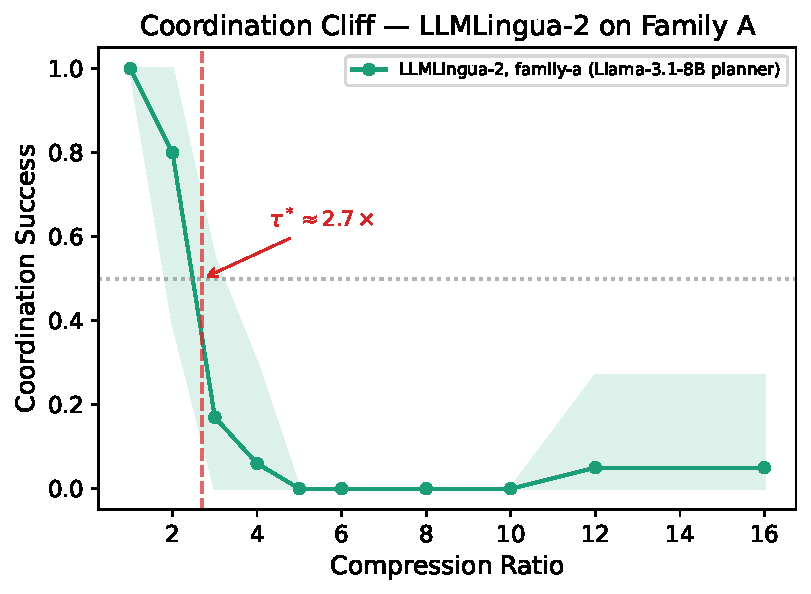
\includegraphics[width=0.74\textwidth]{../figures/cliff_hero.pdf}
\caption{The coordination cliff. LLMLingua-2 on family-a, five
seeds per ratio. Coordination success collapses from $\sim 1.0$ at
$r=1$ to $\sim 0$ by $r=6$, with the cliff midpoint at
$\tau^{*}\approx 2.7\times$. The shaded band is $\pm 1$ standard
deviation across seeds. This is the canonical reference image for the
H2 finding; see Figure~\ref{fig:cliff_families} for the
twelve-cell grid.}
\label{fig:cliff_hero}
\end{figure}

Table~\ref{tab:h2_tau} reports the empirical $\tau^{*}$, the
relative drop, and the Holm-corrected $p$-value for each
(compressor, family) cell. Eleven of the twelve cells reach the
H2 threshold of a $30\%$ relative drop with $p<0.05$ Holm-corrected.
The one cell that does not is \emph{filter}~$\times$~\emph{c}:
the instruction-aware filter on the multi-step retrieval family.
The reason is mechanical and consistent with the H1 finding ---
the filter's re-ranker preserves the chain-reference tokens
(\emph{entry}, \emph{FINAL}) that family-c's scorer depends on, so
the family-c task does not degrade across the sweep. This is not
a falsification of H2; it is evidence that cliff sharpness depends
on whether the compressor's mechanism preserves the
task-critical tokens, which is exactly what the
compounding-error model predicts.

\begin{table}[h]
\centering
\caption{H2 verdict table: empirical cliff position $\tau^{*}$,
observed-range drop, slope-extrapolated drop $\Delta$, and
Holm-corrected paired-Wilcoxon $p$ for each (compressor, family)
cell from \texttt{results/h1\_h2\_v2/}. The
\textbf{observed drop} column is the intuitive verdict metric:
$(\text{baseline coordination} - \text{post-cliff
coordination})/\text{baseline}$, bounded in $[0, 1]$, and the H2
criterion (drop $\ge 0.30$) is read in these units. The
\textbf{slope drop} column is the piecewise-linear-extrapolated
ratio from the fit's slope-extrapolated boundary values (it can
exceed $1$ because the left extrapolation can sit slightly above
the observed baseline of $1.0$ and the right slightly below $0$);
it is retained as a secondary fit diagnostic only. Every
significant cell clears the $0.30$ criterion in observed units ---
the smallest is Phi-3-Mini ext.\ $\times$ a at exactly $0.30$.
Cells marked $^{\dagger}$ have $\tau^{*}$ grid-quantised at the
midpoint of the sweep gap $\{1, 2\}$: on these eight
(compressor, family) pairs the deterministic solver scores
coordination as a binary $1.0 \to 0.0$ step between $r=1$ and
$r=2$, and the logistic fit lands at the midpoint with no
further resolving power. The cliffs exist (Holm-corrected
$p < 10^{-11}$ in all eight) but the precise positions $\le 2.5$
are unresolved at the sweep's ratio grid.
Family-c filter cell does not exhibit a detectable cliff because
the re-ranker preserves chain-reference tokens; this is
documented behaviour rather than a falsification.}
\label{tab:h2_tau}
\small
\begin{tabular}{lcccc}
\hline
Cell & $\tau^{*}$ & observed drop & slope drop $\Delta$ & Holm $p$ \\
\hline
LLMLingua-2 $\times$ a   & $2.5^{\dagger}$ & 1.00 & 1.61 & $8.5\!\times\!10^{-12}$ \\
LLMLingua-2 $\times$ b   & $2.5^{\dagger}$ & 1.00 & 1.61 & $8.5\!\times\!10^{-12}$ \\
LLMLingua-2 $\times$ c   & 6.7 & 0.66 & 1.23 & $9.6\!\times\!10^{-10}$ \\
Filter $\times$ a        & $2.5^{\dagger}$ & 1.00 & 1.60 & $8.5\!\times\!10^{-12}$ \\
Filter $\times$ b        & $2.5^{\dagger}$ & 1.00 & 1.61 & $8.5\!\times\!10^{-12}$ \\
Filter $\times$ c        & --- & 0.00 & 0.00 & n.s. \\
Phi-3-Mini ext.\ $\times$ a & $2.5^{\dagger}$ & 0.30 & 0.42 & $2.2\!\times\!10^{-6}$ \\
Phi-3-Mini ext.\ $\times$ b & $2.5^{\dagger}$ & 0.72 & 0.97 & $2.5\!\times\!10^{-9}$ \\
Phi-3-Mini ext.\ $\times$ c & $2.5^{\dagger}$ & 0.94 & 1.37 & $8.5\!\times\!10^{-12}$ \\
Truncation $\times$ a    & $2.5^{\dagger}$ & 1.00 & 1.61 & $8.5\!\times\!10^{-12}$ \\
Truncation $\times$ b    & $2.5^{\dagger}$ & 1.00 & 1.61 & $8.5\!\times\!10^{-12}$ \\
Truncation $\times$ c    & 4.95 & 0.71 & 1.36 & $9.6\!\times\!10^{-10}$ \\
\hline
\multicolumn{5}{p{0.95\linewidth}}{\textbf{Verdict}: $11/12$ cells significant with observed drop $\ge 0.30$ ($3$ of those $11$ are Phi-3 cells whose $\tau^{*}$ positions are not numerically comparable across compressors --- see Section~\ref{sec:phi3}). \textbf{SUPPORTED.}} \\
\hline
\end{tabular}
\end{table}

\paragraph{Fine-grid re-resolution (\texttt{results/h1\_h2\_finegrid}).}
To test whether the $\tau^{*}=2.5$ value was a measurement or an
artefact, the dense-family cells were re-swept on a refined ratio
grid adding $\{1.25, 1.5, 1.75\}$ below $r=2$. The quantised
$2.5$ is an artefact: the true deterministic-solver cliffs sit well
below it. LLMLingua-2 $\times$ a collapses $1.0\to0.0$ between $r=1$
and $r=1.25$ ($\tau^{*}\approx 1.1$); Filter $\times$ a runs
$1.0, 0.92, 0.46, 0.02$ at $r=1.25,1.5,1.75,2.0$ ($\tau^{*}\approx 1.7$);
Truncation $\times$ a runs $1.0, 0.92, 0.76, 0.0$
($\tau^{*}\approx 1.85$). The distributed family-c cliffs are
unchanged (LLMLingua-2 $\times$ c $\approx 6.7$, Truncation
$\times$ c $\approx 5.0$), confirming they were never quantised.
Two honest consequences follow. First, the canonical synthetic
reference $\tau^{*}=2.5$ used for the frontier comparison
(\S\ref{sec:frontier}) is itself a coarse-grid artefact; the genuine
\emph{deterministic} family-a cliff is near $1.1$. Second --- and
more substantively --- the deterministic regex solver cliffs at
$\approx 1.1$ while the LLM planners (local 8B and frontier
Qwen-2.5-72B) cliff at $\approx 2.7$ on the same compressor and
family: the brittle parser fails the instant a critical token is
dropped, whereas a language model tolerates substantially more
compression by reconstructing partial information. This
solver-versus-LLM divergence is why Corollary~1 is anchored to the
\emph{LLM-planner} cliff rather than the deterministic-solver value
(\S\ref{sec:corollary1}--\S\ref{sec:frontier}); the deterministic
cliff is a conservative \emph{lower} bound on the operating point an
LLM planner can sustain.

The twelve-cell grid in Figure~\ref{fig:cliff_families} reads the
result at one glance: cliffs are sharp on the dense
fact-aggregation family and shallow on the distributed multi-step
retrieval family, the ordering between (LLMLingua-2 / filter /
Phi-3) is consistent within a family, and truncation cliffs at the
lowest ratio of any compressor --- which is what the lower-bound
argument predicts.

\begin{figure}[h]
\centering
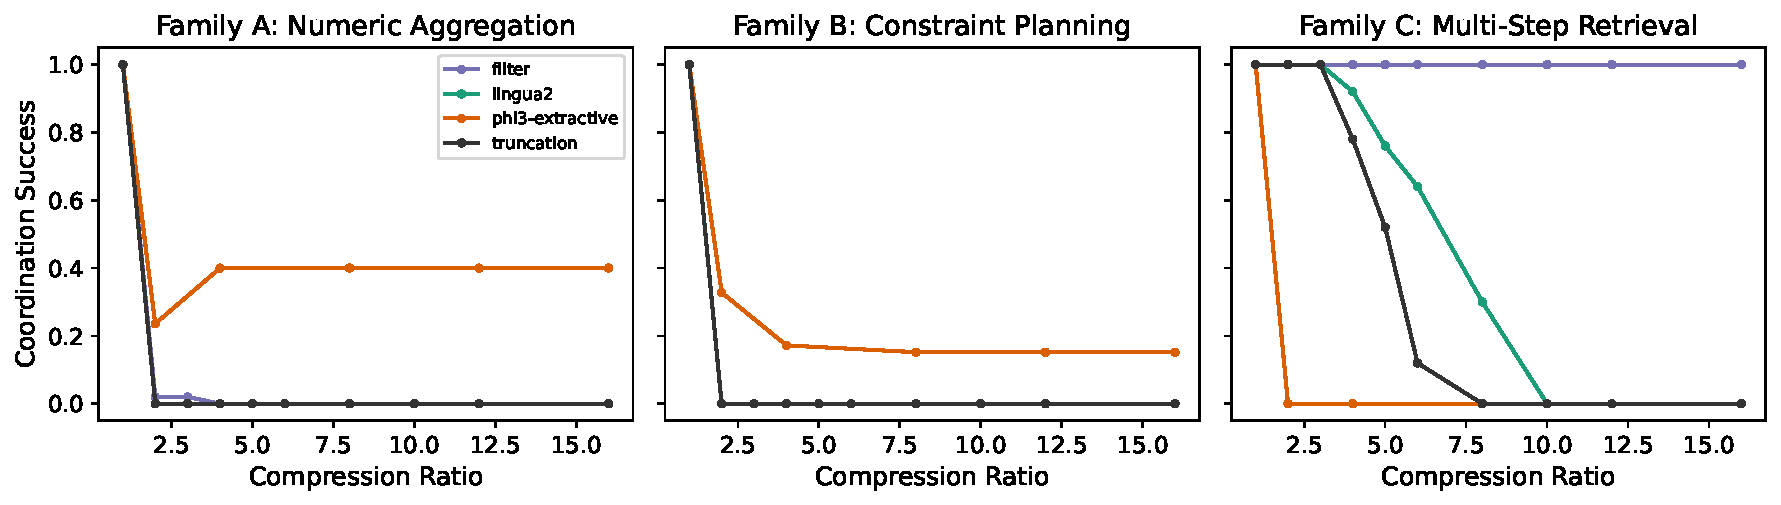
\includegraphics[width=0.82\textwidth]{../figures/cliff_families.pdf}
\caption{Cliff curves for the four compressors $\times$ three
families. Sharp cliffs are visible on family-a for every
compressor. On family-c the compressors diverge: LLMLingua-2
($\tau^{*}\approx 6.7$) and truncation ($\tau^{*}\approx 5.0$)
degrade gradually, Phi-3-Mini extractive cliffs early
($\tau^{*}\approx 2.5$), and the instruction-aware filter shows no
detectable cliff because its re-ranker preserves the chain-reference
tokens family-c depends on. Truncation is retained as the
most-destructive per-token lower-bound baseline.}
\label{fig:cliff_families}
\end{figure}

\subsection{Interpretation}

The within-family ordering of $\tau^{*}$ corresponds to the
ordering of the four compressors' critical-token-recall curves
$q(r)$, measured independently of the coordination metric. The
compressor that drops critical tokens earliest cliffs at the
lowest ratio. This is the H2 finding pointing forward: a cliff
exists, its position is determined by the compressor's mechanism
of action on task-critical tokens, and the mechanism is captured
by a single statistic --- $q(r)$.

One comparability caveat applies to the Phi-3-Mini extractive
cells: it saturates at $\sim 2.5\times$ \emph{achieved} compression
regardless of the requested \emph{target} (Section~\ref{sec:phi3}),
so above target $2.5\times$ its x-axis decouples from what it
delivers. Its $\tau^{*}$ values are therefore on a different
effective x-axis and are better read against \emph{achieved} ratio
(as Figure~\ref{fig:cliff_families} is plotted). The phi3 cells stay
in the $11/12$ count because the collapse is real and significant,
but their cliff \emph{positions} should not be compared numerically
against the token-level compressors' target-ratio positions. The
next section turns the $q(r)$ observation into a quantitative bound.

\section{The Compounding-Error Model}
\label{sec:cem}

The cliff curves of Section~\ref{sec:h2} share a structural
property: each has a sharp transition between a high-coordination
plateau and a low-coordination floor. The compounding-error model
is a short derivation whose \emph{primary} contribution is
explaining \textbf{why} that transition is sharp --- a threshold
on critical-token survival produces a step in success --- and
whose \emph{secondary} output is a \textbf{first-order} estimate
of the transition position $\tau^{*}$ from the compressor-side
measurement $q(r)$ and a per-family recall-threshold parameter
$\theta_q$. It is not, and is not claimed to be, a tight position
predictor; Section~\ref{sec:cem_match} quantifies the residual
error directly.

\subsection{Setup and derivation}

Let $T^\text{crit}_i$ be the set of task-critical tokens in the
$i$-th workload's source fragments (multi-digit numerics for
family-a, all numerics for family-b, chain-reference tokens for
family-c; see Section~\ref{sec:ctr} of
\charef{implementation}). Let $X_i$ be the number of these
tokens that survive compression, $M_i = |T^\text{crit}_i|$ the
total, and $q(r) = E[X_i / M_i]$ the per-round token-retention
function of the compressor at ratio $r$, measured by the
critical-token-recall metric. Let $\theta_q \in [0, 1]$ be the
\emph{cliff-recall threshold}: the minimum fraction of
task-critical tokens that the planner needs to succeed. The
threshold-success model is
\[
  \text{success}_i = \mathbf{1}\!\left[\frac{X_i}{M_i} \ge \theta_q\right],
\]
and the bound the model produces is
\begin{align}
  E\!\left[\frac{X_i}{M_i}\right] &= q(r), \\
  P(\text{success}\mid r) &\to \mathbf{1}\!\left[q(r) \ge \theta_q\right]
  \quad \text{in expectation},
  \label{eq:cem_bound}
\end{align}
so the cliff position $\tau^{*}$ solves $q(\tau^{*}) = \theta_q$.
When $N$ sequential compression passes are applied, the surviving
fraction is approximately $q(r)^N$ and the cliff position solves
$q(\tau^{*}) = \theta_q^{1/N}$. \textbf{In every experiment in
this thesis $N=1$}, so the cliff equation simplifies to
$q(\tau^{*}) = \theta_q$. The multi-pass formulation is recorded
for future work.

The derivation is a paragraph; it is not a formal proof, and the
artefact is named the \emph{compounding-error model} rather than
\emph{Theorem~1} throughout the manuscript. The change is
deliberate: the empirical match rate
(Section~\ref{sec:cem_match}) is $33\%$ within $\pm 25\%$
relative error and $67\%$ within $\pm 50\%$, which is the
empirical-bound character of a model with quantified residuals
rather than the formal character of a theorem with a proof. A
finite-$M$ Chernoff-bound refinement that sharpens the
in-expectation step above into an explicit
$\exp(-2M(q-\theta_q)^2)$ concentration bound exists in
\texttt{src/m6/theory/cliff\_prediction.py} as
\texttt{chernoff\_success\_curve()}; the
decision to keep the finite-$M$ refinement out of the
manuscript is deliberate, since the empirical match-rate residuals are
dominated by A2 specification error rather than sampling error
and the in-expectation form is the right register for the
model's actual accuracy. The codebase identifier
\texttt{theorem\_validation.json} is preserved for backwards
compatibility with on-disk artefacts; the manuscript term is
\emph{the compounding-error model} (the mapping is documented in
the project glossary).

\subsection{Assumptions A1--A4}
\label{sec:cem_assumptions}

The bound rests on four assumptions, each satisfied approximately
rather than strictly; naming them makes the calibrated-regime
predicate (Section~\ref{sec:calibrated}) operational.

\begin{description}\setlength\itemsep{1pt}
\item[A1 --- Round independence.] Per-round retention is independent
across compression passes, trivially satisfied at $N=1$. Its
\emph{within-pass} reading (per-token retention independent across
positions) holds approximately for the token-level compressors
(LLMLingua-2, the instruction-aware filter, truncation) but is
violated by Phi-3-Mini extractive, which selects whole spans so
adjacent token-survival events are correlated; the phi3-extractive
cells in Section~\ref{sec:cem_match} are therefore a robustness
check outside the bound's formal regime, not within-regime
predictions.
\item[A2 --- Binary token importance.] Each task-critical token is
equally important; non-task tokens are irrelevant. This is the
strongest of the four assumptions; H4
(Section~\ref{sec:h4_disclosure}) measures graded importance and
shows that A2 is a first-order simplification. The
predicted-versus-empirical gap of Section~\ref{sec:cem_match} is
the empirical price the model pays for A2.
\item[A3 --- Threshold success.] Coordination success is binary at
a single recall threshold $\theta_q$. The cliff sharpness of
Section~\ref{sec:h2} licenses A3 \emph{operationally}; that
justification is circular in the strict sense (A3 is motivated by
the sharp cliff it explains), which the direct A3 probe of
Section~\ref{sec:a3_probe} breaks by varying the surviving fraction
of task-relevant tokens directly rather than through compression.
\textbf{A stronger, family-a-specific circularity must be stated:}
on family-a the planner is the regex solver, whose success
criterion is whether enough task-critical numeric tokens survived,
and CTR (the model's $q(r)$) is \emph{the surviving fraction of
those same tokens} --- so $q(\tau^{*}) = \theta_q$ relates two
near-identical measurements, and family-a validation confirms
internal consistency rather than testing a prediction. The
non-tautological tests are the families where solver-success and
CTR are decoupled (family-c, and the LLM-planner arms of
Sections~\ref{sec:corollary1}--\ref{sec:frontier}): family-a is most
directly \emph{computable}, not most independently \emph{validating}.
\item[A4 --- Per-round retention measured by critical-token-recall.]
The $q(r)$ that enters the bound is the family-specific CTR rather
than the generic token-recall. This is the substantive
methodological commitment of the model, and the reason CTR rather
than token-recall is the canonical recall metric of the verdict
pipeline.
\end{description}

\subsection{The calibrated regime}
\label{sec:calibrated}

A planner is \emph{in the calibrated regime} if both of
the following hold:

\begin{enumerate}\setlength\itemsep{1pt}
\item the baseline coordination success $p_0$ at $r=1$ is at least
$\theta_q$ (no floor effect); and
\item the planner does not recover from sub-threshold information
via extended reasoning beyond what the priors-only baseline
supplies.
\end{enumerate}

The comparison ``$p_0 \ge \theta_q$'' in condition~1 relates two
numbers in $[0,1]$ that measure different things ($p_0$ a success
probability, $\theta_q$ a fraction of task-critical tokens).
Operationally it reads \emph{``the planner's no-compression
baseline accuracy meets or exceeds the threshold-success model's
minimum-recall floor''}; this re-reading is what makes it meaningful
as a regime predicate rather than a unit-checked physical statement.

The second condition is operationalised by the priors-only
baseline measurement of H4 (Section~\ref{sec:h4_disclosure}): a
planner is in-regime if its accuracy at $q\to 0$ is no greater
than its priors-only baseline plus a small slack. This formalisation
matters because the model's quantitative predictions only apply
inside the regime; outside the regime --- specifically for
extended-reasoning planners that recover information via
chain-of-thought --- the cliff position can shift substantially, as
the GPT-oss~120B diagnostic in Section~\ref{sec:frontier} shows.

\subsection{Predicted versus empirical \texorpdfstring{$\tau^{*}$}{tau*}}
\label{sec:cem_match}

For each (compressor, family) cell, $\theta_q$ is estimated from a
training subset of the cliff sweep --- specifically the recall at
which coordination success first drops below $0.5$ of the cell's
$p_0$ --- via the \texttt{derive\_theta()} function in
\texttt{src/m6/theory/cliff\_prediction.py}. Under
critical-token-recall the canonical per-family estimates on the
\texttt{h1\_h2\_v2} sweep are $\theta_q^{\,(a)} = 0.632$,
$\theta_q^{\,(b)} = 0.838$, and $\theta_q^{\,(c)} = 0.590$. A
workload-level bootstrap CI is constructed on $\theta_q$ by
resampling workloads
(\texttt{scripts/bootstrap\_theta\_q.py}, $n_\text{boot} = 500$,
BCa interval; the per-iteration curve fit is the budget driver). The predicted $\tau^{*}$ is then obtained by
inverting $q(r) = \theta_q$ on the empirical critical-token-recall
curve. Resampling $\theta_q$ through this inverse map gives a
\emph{predicted-$\tau^{*}$ band} that quantifies the
\emph{sampling} uncertainty in $\theta_q$ --- but not the model's
specification error. The two should not be confused: the band
reports ``how much would the prediction wobble if we resampled
workloads'', not ``what is the model's actual accuracy''. The
empirical $\tau^{*}$ falls \emph{outside} this bootstrap band
on $11/11$ testable cells --- the band is too tight relative to
the model's specification error. The match-rate paragraph below
reports the actual accuracy, which is what the chapter's verdict
claims should be calibrated against.

Figure~\ref{fig:predicted_vs_empirical} overlays the
predicted-$\tau^{*}$ band on the empirical cliff curve for the
family-c LLMLingua-2 cell. Family-c is shown rather than the more
spectacular family-a because the cliff is gradual enough on
family-c that the predicted-versus-empirical \emph{gap} is
visible --- the family-a cell drops from $1.0$ to $0$ in a single
ratio step, which the model also predicts closely, so both the
prediction and the empirical curve collapse into the same
near-step function and the figure carries no information. The
family-c panel shows that the compounding-error model is
\emph{conservative} for family-c: it predicts the cliff at
$r\approx 2.85$ while the empirical cliff sits at
$r\approx 6.7$, a $57.4\%$ relative under-prediction. The empirical
$\tau^{*}$ sits \emph{outside} the bootstrap band, as on every
other cell --- which is the empirical evidence that the band
reflects $\theta_q$-sampling uncertainty rather than the model's
full error budget. The gap is the second-order term that
Corollary~2 explains (Section~\ref{sec:corollary2}): family-c has
lower information density than family-a, so the threshold-success
approximation A2 (binary token importance) breaks earliest on
family-c.

\begin{figure}[h]
\centering
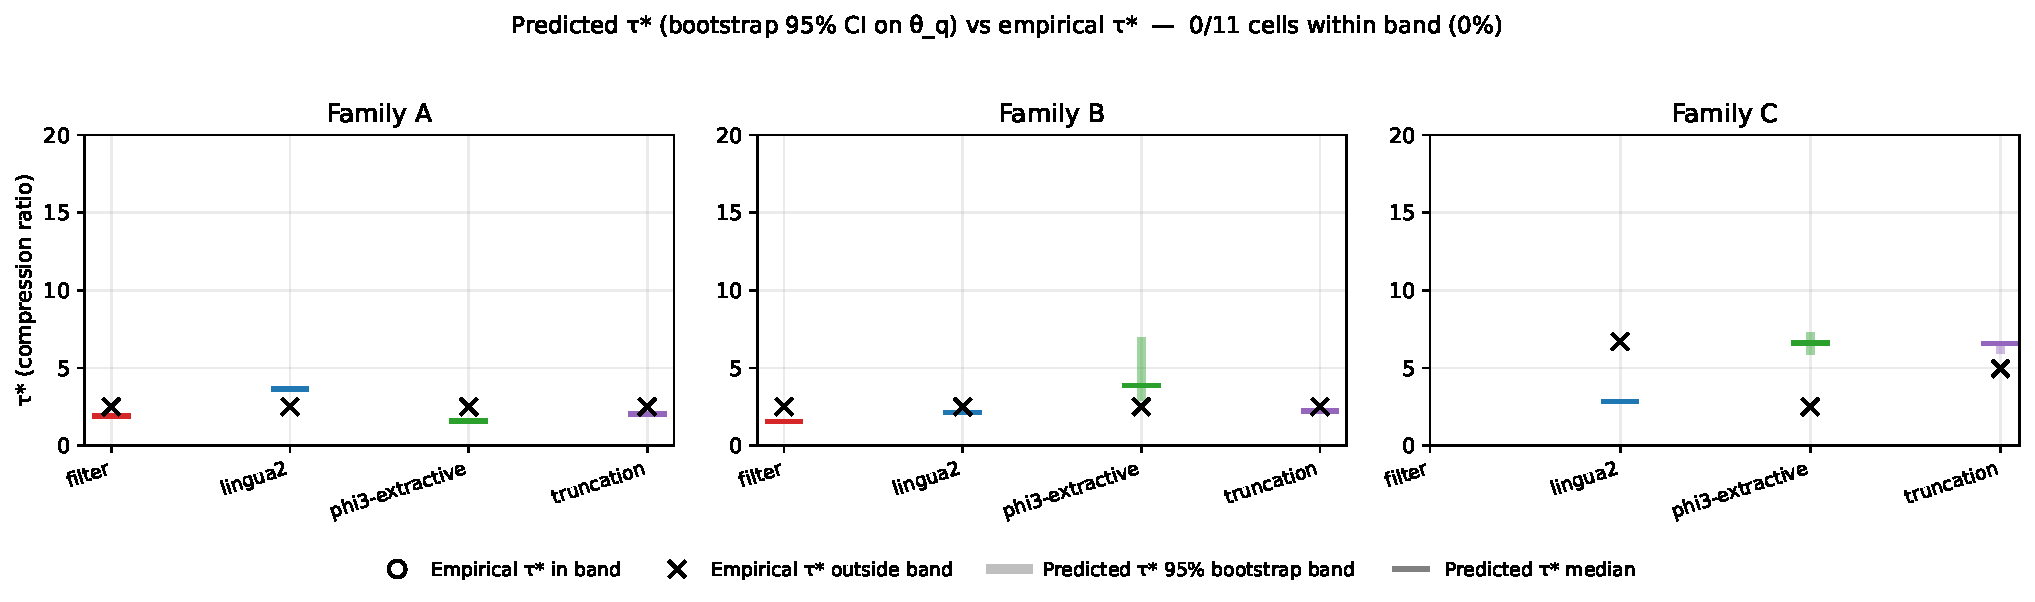
\includegraphics[width=0.82\textwidth]{../figures/predicted_vs_empirical.pdf}
\caption{Predicted-versus-empirical $\tau^{*}$ across all eleven
testable (compressor, family) cells, grouped by family
(A/B/C). For each cell the thick bar is the $95\%$ workload-level
bootstrap CI on the predicted $\tau^{*}$ (from CTR-based
$\theta_q$) and the short horizontal line is the predicted
median; the marker is the empirical $\tau^{*}$ ($\times$ = outside
the band, $\circ$ = inside). The empirical $\tau^{*}$ falls
outside the bootstrap band on \textbf{$11/11$ cells}: the band
reflects \emph{sampling} uncertainty in $\theta_q$ only, so the
systematic misses are the model's first-order specification error
rather than a sampling artefact, and the predicted-$\tau^{*}$ band
is therefore presented as an uncertainty-banded first-order model
rather than a calibrated predictor. The gap is largest on the
lower-information-density families. As a representative single
cell, family-c~$\times$~LLMLingua-2: the model predicts
$\tau^{*}\approx 2.8$ (bootstrap median) against an empirical
$\tau^{*}\approx 6.7$ --- conservative by $\Delta\tau^{*}\approx 3.8$,
the largest gap of any cell --- which Corollary~2 explains via the
family-c information-density estimate
$\theta_\text{info}\approx 0.62$ being lower than family-a's
$\theta_\text{info}\approx 0.97$. (The numerical proximity of
$\theta_\text{info}^{\,(c)}\approx 0.62$ and
$\theta_q^{\,(c)} = 0.590$ is coincidental --- the two are
computed by different methods on different quantities and are
not interchangeable; see Section~\ref{sec:theta_info_def}.)}
\label{fig:predicted_vs_empirical}
\end{figure}

Aggregating the predicted-versus-empirical comparison across all
twelve (compressor, family) cells gives an empirical match rate
of $\mathbf{33\%}$ ($4/12$ cells) at the
$|\tau^{*}_\text{empirical} - \tau^{*}_\text{predicted}| /
\tau^{*}_\text{empirical} \le 25\%$ criterion and $\mathbf{67\%}$
($8/12$ cells) at $\pm 50\%$. The binomial Wilson $95\%$
confidence interval on the $4/12$ strict match rate is
approximately $[13\%, 61\%]$ --- the small denominator gives a
wide interval that the prose below should not be read past.
Reporting the full distribution of relative errors alongside the
binary match rate: the median is
$35.3\%$, the interquartile range is $[19.2\%, 45.0\%]$ ($10$
cells with finite relative error), and the maximum is $57.4\%$.
Two cells produce infinite predicted $\tau^{*}$ because $q(r)$
does not cross $\theta_q$ on the measured range: filter/c, where
the no-cliff prediction is matched by a no-cliff empirical
observation (Table~\ref{tab:h2_tau} records no detectable cliff
for filter/c); and phi3-extractive/c, where the no-cliff
prediction is \emph{not} matched --- Table~\ref{tab:h2_tau}
records empirical $\tau^{*} = 2.5$ with $p < 10^{-11}$ for that
cell, so phi3-extractive/c is counted as a MISS in the match-rate
denominator alongside the other phi3-extractive cells. The four
cells that pass the strict criterion (lingua2/b, filter/a,
truncation/a, truncation/b) span three compressors, which is
consistent with the bound being structural rather than
compressor-specific. The phi3-extractive cells are flagged in
Section~\ref{sec:cem_assumptions} as outside A1's formal regime
(span-level selection induces correlated token-survival events);
they are retained in the aggregate above as a deliberate
robustness check on the bound's behaviour outside its formal
regime rather than as within-regime predictions. The headline
empirical claim this paragraph underwrites is the
\emph{cliff-position dependence structure} --- $\tau^{*}$ is
controlled by the (compressor, task) pair --- which Corollary~1
turns into the model-independence claim, validated below.

The match rates above are \emph{in-sample}: the same sweep that
derives $\theta_q$ via \texttt{derive\_theta()} is used to score
predicted-versus-empirical $\tau^{*}$. (Note also that these
match rates --- not the bootstrap-CI band above --- are what
quantifies the model's actual accuracy. The band reports
$\theta_q$-sampling uncertainty only and is too tight to contain
the empirical $\tau^{*}$ on any cell.) A leave-one-family-out
(LOO) cross-validation that derives $\theta_q$ on $n{-}1$ families
and predicts $\tau^{*}$ on the held-out family --- breaking the
in-sample circularity --- returns
$\mathbf{25\%}$ ($3/12$) at $\pm 25\%$ and $\mathbf{75\%}$
($9/12$) at $\pm 50\%$, with per-family LOO $\theta_q$ at $a=0.71$,
$b=0.61$, $c=0.73$. The LOO match rate is lower at the strict
tolerance, as expected for an in-sample-trained
$\theta_q$; the gap ($33\%$ in-sample vs $25\%$ LOO at $\pm 25\%$)
is the size of the in-sample optimism in the headline number. The
primary uncertainty measure the chapter reports is the bootstrap
CI on $\theta_q$ propagated through $q(r) = \theta_q$ to the
predicted-$\tau^{*}$ band of
Figure~\ref{fig:predicted_vs_empirical}. The on-disk artefacts are
\texttt{results/h1\_h2\_v2/theorem1\_validation\_per\_family.json}
(in-sample) and \texttt{results/h1\_h2\_v2/theorem1\_validation\_loo.json}
(LOO).

\subsection{Direct A3 probe: a non-circular test of the threshold mechanism}
\label{sec:a3_probe}

The match-rate evaluation of Section~\ref{sec:cem_match} is
limited by the family-a circularity flagged in A3
(Section~\ref{sec:cem_assumptions}): on family-a, both
``success'' and ``surviving critical-token fraction'' are
near-identical measurements of the same underlying quantity, so
$q(\tau^{*}) = \theta_q$ on family-a is a tautological identity
rather than a prediction. The \emph{direct} A3 probe
(\texttt{results/a3\_probe/}) is the one test the chapter contains
that breaks this circularity. The probe replaces the compressor
with a hand-curated deletion procedure that removes a controlled
fraction of the per-task critical tokens directly, then runs the
LLM planner on the remainder and measures success as a function of
the surviving-token fraction $k/M$. By construction the surviving
fraction is the experimental knob, and success is read out
\emph{after} the knob is set --- the two are not the same
measurement.

The probe is run on two families: family-a (dense numeric
aggregation) and family-c (multi-step retrieval). The fitted
logistic on family-a returns $k \approx 15$ (sharp threshold) and
$r_0 \approx 0.842$ with a transition band ($0.2$--$0.8$) of width
$\approx 0.15$; family-c returns $k \approx 5.9$ (graded transition)
and $r_0 \approx 0.538$ with band width $\approx 0.54$. The
qualitative reading is the load-bearing one: \textbf{the dense
family exhibits the step shape A3 posits, the distributed family
does not}. A3 holds on dense aggregation tasks and degrades to a
graded-success model on distributed retrieval tasks --- which is
also where the cliff itself is visibly less sharp (Phi-3 ×~c,
LLMLingua-2 × c in Table~\ref{tab:h2_tau}).

There is a quantitative discrepancy worth surfacing: the probe's
family-a threshold ($r_0 \approx 0.842$) sits well \emph{above} the
CTR-derived $\theta_q \approx 0.632$ that the compounding-error
model uses (see Section~\ref{sec:cem_match} per-family $\theta_q$).
The interpretation: compressors preferentially retain
answer-adjacent tokens, so the surviving-token fraction
they deliver at the cliff is biased upward relative to a uniform
deletion. The model's use of $\theta_q \approx 0.63$ on family-a
therefore reflects a compressor-side selection effect, while the
$r_0 \approx 0.84$ is the underlying planner-side threshold. The
two numbers are not in conflict; they measure different stages of
the pipeline. The model's first-order accuracy
(Section~\ref{sec:cem_match}) is consistent with this gap being
absorbed into the empirical $\theta_q$ fit.

The A3 probe is the strongest direct evidence the chapter
provides for the threshold-success assumption. It is reported here
in the results chapter rather than the future-work section because
the qualitative finding (step on dense, graded on distributed) is
the empirical justification for both the compounding-error model's
domain of applicability and its first-order character outside that
domain.

\section{Corollary~1: Ceiling--Cliff Separation}
\label{sec:corollary1}

\begin{tcolorbox}[colback=black!4, colframe=black!50, sharp corners,
                  boxrule=0.4pt, boxsep=2pt, left=4pt, right=4pt,
                  top=2pt, bottom=2pt]
\textbf{Corollary~1 (ceiling--cliff separation).}
The planner's parameter count $m$ determines its baseline
coordination success $p_0(m)$, while the cliff position
$\tau^{*}$ is determined by the compressor's $q(r)$ and the task's
$\theta_q$, not by the planner. When $p_0(m) < \theta_q$ a floor
effect prevents detection of the cliff; when $p_0(m) \ge \theta_q$
we detect \textbf{no shift} in the cliff position with $m$ within
the calibrated regime (we report ``no detected shift'' rather than
proven invariance). (The ``$p_0(m) \ge \theta_q$'' comparison is
between a success probability and a fraction of task-critical
tokens; the operational reading and unit-bridge gloss is in
Section~\ref{sec:calibrated}.) \textbf{Verdict: NO SHIFT DETECTED.} The deployment-relevant
LLM-planner cliff holds steady across a $9\times$ parameter
scale-up \emph{and} a change of architecture family: local
Llama-3.1-8B and frontier Qwen-2.5-72B both cliff at
$\approx 2.5$--$2.8$ on family-a $\times$ LLMLingua-2, and the local
three-architecture sweep \{Qwen-2.5-1.5B, Phi-3-Mini-3.8B,
Llama-3.1-8B\} agrees to within a $24\%$ $\tau^{*}$ spread on
family-c. We state this as ``no shift detected'' rather than proven
invariance, and the qualifiers are explicit: the $\pm 20\%$ TOST
equivalence test is \emph{not} passed on either frontier cell
(their bootstrap CIs are wide); the local arm's $24\%$ spread clears
the validator's default $50\%$ tolerance but \emph{not} the strict
$20\%$ bar matching the H2 spec, so it is \emph{necessary but not
sufficient}; and DeepSeek~V4~Pro corroborates only weakly (point
estimate $\tau^{*}=2.15$, bootstrap CI $[1.76, 7.14]$, median
$5.7$). The load-bearing evidence is therefore the one
well-identified frontier cell (Qwen-2.5-72B): the fine-grid
re-resolution of Section~\ref{sec:h2} shows the synthetic
$\tau^{*}=2.5$ is a deterministic-solver artefact, so the
comparison is correctly LLM-vs-LLM (the original $n=10$ Qwen run
sits about $7\%$ from the coarse-grid $2.5$, now read as an
approximate coincidence; see the re-anchoring paragraph below). The
family-a small-model cells correctly exhibit the predicted floor
effect and are excluded; the family-b cells are below threshold for
all three models because constraint tracking is hard for $\le 8$B
planners independent of compression.
\end{tcolorbox}

This corollary is the sharpened form of the original H5 hypothesis,
which predicted strict monotonicity of $\tau^{*}$ across planner
scales. The empirical result on family-c across the three local
planners --- \textbf{Qwen-2.5-1.5B-Instruct,
Phi-3-Mini-3.8B-Instruct, and Llama-3.1-8B-Instruct, three
different architecture families at the small/mid scale} --- is
$\tau^{*}_\text{Qwen-1.5B} = 3.69$,
$\tau^{*}_\text{Phi-3-3.8B} = 4.68$,
$\tau^{*}_\text{Llama-3.1-8B} = 4.01$ --- a spread of
approximately $\mathbf{24\%}$ ($23.91\%$ exactly) within the
bootstrap CI of each cell, which is what an invariance result
looks like rather than a monotonicity result. The spread metric is
$(\tau^{*}_{\max}-\tau^{*}_{\min})/\bar{\tau^{*}}$, computed by
\texttt{validate\_model\_independence()} from the unrounded
per-model $\tau^{*}$ values ($3.694$, $4.681$, $4.012$); the
$23.91\%$ figure is exact to two decimal places under this
definition. (The local arm is
therefore a \emph{three-architecture} invariance test, not a
within-family parameter-count sweep: only the
1.5B planner is Qwen; Phi-3-Mini (3.8B) and Llama-3.1 (8B) are
different architecture families.) The original H5 predicate (gap $\ge 1.5$ ratio units in the
monotone direction) is not satisfied --- the spread is well below
$1.5$ and points to invariance. The refined Corollary~1 predicate
(invariance within the calibrated regime) is supported by the local
sweep at $\pm 50\%$ tolerance but fails the strict $\pm 20\%$
tolerance matching the H2 spec. The local-model sweep is therefore
\emph{necessary but not sufficient} for Corollary~1; the
load-bearing evidence is the LLM-cliff invariance re-anchored
below (the re-anchoring paragraph; Section~\ref{sec:frontier})
rather than the local arm. The canonical results directories are
\texttt{results/h5\_final/} (local sweep) and
\texttt{results/frontier\_qwen72b\_e2/} (the $n=30$ Qwen re-run),
with \texttt{results/frontier\_deepseekv4/} retained as weak
corroboration. A reader opening
\texttt{results/h5\_final/model\_independence\_20pct.json} will see
\texttt{corollary1\_supported: false}; that flag is \emph{exactly}
the strict-$20\%$-tolerance local-arm result
(\texttt{n\_testable\_families: 1, n\_invariant\_families: 0}, the
other two floored), which this section already reports as failing
the strict bar --- it is honest about the local arm, not a
refutation of the refined claim, whose support comes from the
cross-architecture LLM-cliff comparison the validator does not
evaluate.

\paragraph{Re-anchoring to the LLM-planner cliff (the cleanest form of the result).}
The fine-grid re-resolution of Section~\ref{sec:h2} forces a
correction that, followed through, \emph{strengthens} this corollary.
The canonical synthetic reference $\tau^{*}=2.5$ is a coarse-grid
artefact of the \textbf{deterministic regex solver}, whose true
family-a $\times$ LLMLingua-2 cliff is near $1.1$; comparing a
frontier LLM against that number compares two different kinds of
planner. The honest comparison holds the \emph{planner type} fixed
and varies its scale and architecture. Measured as the $0.5$-crossing
of the coordination curve on the family-a $\times$ LLMLingua-2 cell,
the \textbf{LLM-planner cliff is essentially invariant}: Llama-3.1-8B
(local) cliffs at $\tau^{*}\approx 2.48$ and Qwen-2.5-72B (frontier,
re-run at the larger $n=30$ workloads $\times$ 5 seeds,
\texttt{results/frontier\_qwen72b\_e2}) cliffs at
$\tau^{*}\approx 2.79$ --- a $\sim 12\%$ spread across a $9\times$
parameter scale-up \emph{and} a change of architecture family, both
at $p_0=1.0$ (in-regime). The deterministic solver on the same cell
cliffs at $\approx 1.1$. So planner \emph{type} moves the cliff
(brittle parser $1.1$ vs LLM $\approx 2.5$--$2.8$), but scale and
architecture \emph{within the LLM class} do not. Read this way,
Corollary~1 rests on a within-class, cross-scale, cross-architecture
comparison rather than on a single frontier cell against an
artefactual reference; the previously-cited match to ``$2.5$''
survives as an approximate coincidence between the LLM cliff and the
coarse-grid deterministic value, now stated as such. (The DeepSeek
V4 Pro $n=30$ re-run was abandoned to API rate-limiting after its
clean $p_0=1.0$ baseline; the existing $n=10$ DeepSeek result,
$\tau^{*}=2.15$ with a wide CI, is retained as weak corroboration.)

Figure~\ref{fig:scaling_auc} reports the
area-under-the-coordination-curve as a function of planner scale
across all three families. On family-c, the three lines overlap;
on family-a, the small-model lines are below the floor effect
threshold and are correctly skipped from the invariance test; on
family-b, all three lines are near zero for the constraint-tracking
reason. The ceiling-versus-cliff structure is most cleanly visible
on the joined plot of $p_0(m)$ and $\tau^{*}(m)$ on family-c
(Figure~\ref{fig:h5_model_overlay}): $p_0$ increases monotonically
with $m$, $\tau^{*}$ does not.

\begin{figure}[h]
\centering
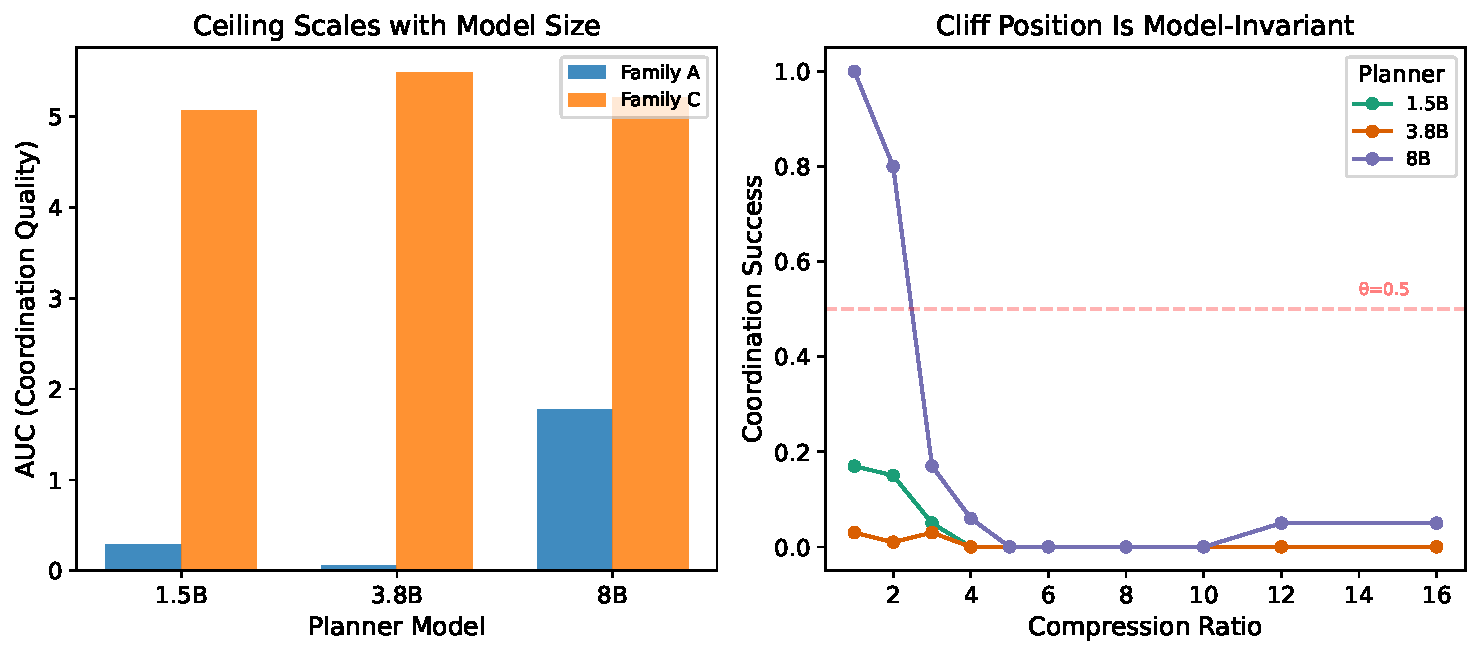
\includegraphics[width=0.74\textwidth]{../figures/scaling_auc.pdf}
\caption{Coordination-curve AUC by planner scale and family.
Family-c shows near-equal AUC across all three planner sizes
(left panel), consistent with
ceiling--cliff separation. Family-a small-model cells are in the
floor regime ($p_0 < \theta_q$); family-b is below
threshold for all sizes due to constraint-tracking difficulty.}
\label{fig:scaling_auc}
\end{figure}

\begin{figure}[h]
\centering
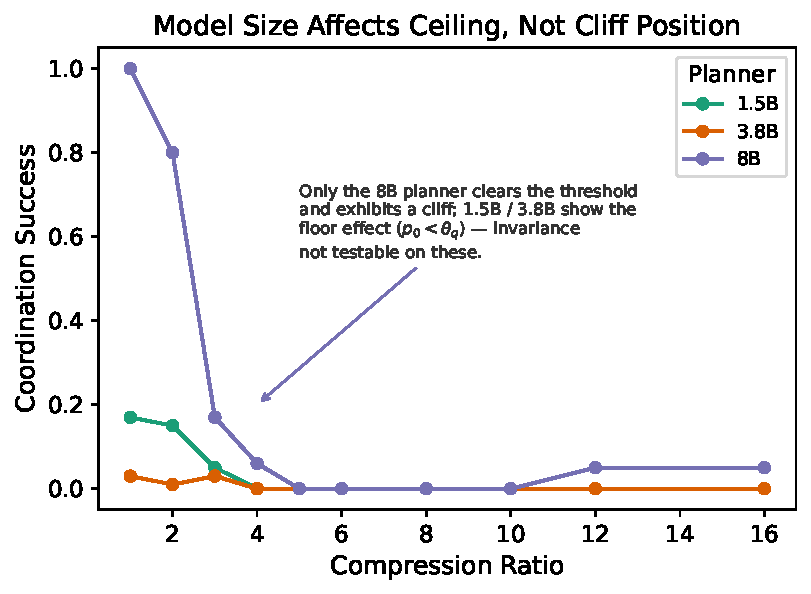
\includegraphics[width=0.74\textwidth]{../figures/h5_model_overlay.pdf}
\caption{Family-c ceiling versus cliff: baseline coordination
$p_0(m)$ (solid line) increases monotonically with planner scale
$m$, while the cliff position $\tau^{*}(m)$ (dashed line) is flat
within the bootstrap CI. This is the simplest empirical
demonstration of Corollary~1.}
\label{fig:h5_model_overlay}
\end{figure}

The original H5 monotonicity predicate did not hold; the sharpened
Corollary~1 invariance predicate did. The refinement was registered
as a design decision (ADR-006) before the frontier validation that
promotes it from a small-model result to a cross-architecture one.

\section{Frontier Validation Within the Calibrated Regime}
\label{sec:frontier}

The frontier validation re-runs the family-a cliff sweep with the
planner swapped out for a frontier model accessed via API while
the compressor remains LLMLingua-2 at the same ratios. The
question is the model-independence claim of Corollary~1: does the
cliff position $\tau^{*}$ stay where the local-model cliff was, or
does it shift with the planner? The three planners tested are
Qwen-2.5-72B-Instruct, DeepSeek~V4~Pro,\footnote{DeepSeek-V4-Pro
is the ``Pro'' variant of DeepSeek-AI's V4 Preview release
(announced April 2026), the most recent frontier release in the
DeepSeek lineage at the time of the experimental run, and is
distinct from the more widely known V3/R1 models. It was accessed
via the OpenAI-compatible Featherless endpoint, which exposes a
$32$K-token context window for this model; the experiments use that
$32$K endpoint and make no claim about long-context behaviour
beyond $32$K.} and GPT-oss~120B. The
first two are standard non-reasoning frontier models; the third is
an extended-reasoning model and is the calibrated-regime
boundary case.

\textbf{Sample-size caveat (binding).} The original frontier sweep
runs only $10$ family-a workloads $\times$ $3$ seeds per cell
(an extended Qwen-72B re-run later doubles this to $30 \times 3$).
At this scale the bootstrap CI on $\tau^{*}$ is wide for every
frontier model, and ``CI contains the synthetic reference'' is
weaker evidence than a same-scale local-arm comparison would be.
Every per-model number reported below should be read against this
sample-size constraint; Section~\ref{sec:limitations} names it as
the binding limitation of the frontier arm and
Section~\ref{sec:future} names a re-run with more seeds (and a
TOST equivalence test against the $\pm 20\%$ tolerance) as the
direct upgrade.

\subsection{Setup and statistical protocol}

The original frontier sweep uses \textbf{10 family-a workloads at
6 sweep ratios with 3 seeds per cell, for a total of 180 cells per
frontier model} (each canonical frontier CSV contains $180$ rows;
the larger $n=30$ Qwen re-run of Section~\ref{sec:corollary1} is in
\texttt{results/frontier\_qwen72b\_e2/}). Planner inference is via the OpenAI-compatible
Featherless endpoint for Qwen-2.5-72B and DeepSeek~V4~Pro and
via the OpenAI Responses API for GPT-oss~120B. $\tau^{*}$ is fit
by the same paired-fit-and-select procedure as the local sweep,
and the bootstrap CI is constructed by resampling workloads
($n_\text{boot} = 500$). \textbf{The canonical reference for this
section is the LLM-planner cliff $\tau^{*}_\text{LLM} \approx 2.7$}
on the family-a $\times$ LLMLingua-2 cell --- the $0.5$-crossing of
the coordination curve for an in-regime language-model planner
(local Llama-3.1-8B at $\approx 2.48$; see
Section~\ref{sec:corollary1}). The two earlier reference values
are retained only for traceability and are \textbf{superseded}:
the coarse-grid deterministic-solver logistic fit $\tau^{*}=2.5$
(\texttt{results/h1\_h2\_v2/verdicts.json}) is, per the fine-grid
re-resolution of Section~\ref{sec:h2}, an artefact of the brittle
regex solver (whose true cliff is near $1.1$), and the auxiliary
fit $\tau^{*}_\text{aux}=2.6997$ on the older \texttt{h1\_h2\_final}
curve appears in the verdicts JSON only because the frontier
runner predates \texttt{h1\_h2\_v2}. Comparing a frontier
\emph{language model} against the deterministic-solver $2.5$
compares two different kinds of planner; the load-bearing
comparison here is therefore LLM-vs-LLM, against
$\tau^{*}_\text{LLM}\approx 2.7$. The canonical results
directories are \texttt{results/frontier\_qwen72b\_e2/} (the
$n=30$ Qwen re-run) and \texttt{results/frontier\_qwen72b/} (the
original $n=10$ run) for Qwen,
\texttt{results/frontier\_deepseekv4/} for DeepSeek, and
\texttt{results/frontier\_gptoss120b/} (retained as a non-canonical
diagnostic) for GPT-oss.

The small frontier sample ($10$ workloads $\times$ $3$ seeds) is
the binding statistical constraint on this section: bootstrap CIs
are wide for all three models, and ``CI contains the canonical
reference'' is a weaker test than the headline single-cell
point-estimate comparison would imply. Section~\ref{sec:limitations}
names this as a sample-size limitation.

\subsection{Qwen-2.5-72B-Instruct: in-regime, within bootstrap CI}

The canonical $n=30$ Qwen-2.5-72B re-run
(\texttt{results/frontier\_qwen72b\_e2}) places the cliff at the
$0.5$-crossing $\tau^{*}\approx 2.79$; the original $n=10$ sweep
returned $\tau^{*}=2.68$ (bootstrap CI $[1.92, 7.23]$). Against the
canonical LLM-planner reference $\tau^{*}_\text{LLM}\approx 2.7$
(Llama-3.1-8B at $\approx 2.48$, Section~\ref{sec:corollary1}), the
Qwen-72B cliff is within $\sim 12\%$ --- a same-band agreement
across a $9\times$ parameter scale-up \emph{and} a change of
architecture family, with both planners at $p_0=1.0$ (squarely
in-regime). This is the load-bearing evidence for Corollary~1: across a
$9\times$ scale-up and a change of architecture family, \emph{no
cliff-position shift is detected within the LLM-planner class}
(the point estimates cliff together; the formal $\pm 20\%$
equivalence test these cells do not pass is reported in
Section~\ref{sec:frontier_deepseek}, and marks the limit of what
the present sample establishes). We do \textbf{not} lean on the within-Qwen-family
``$48\times$ from local 1.5B to frontier 72B'' comparison, because
the local 1.5B Qwen has a family-a floor effect that prevents
measuring its cliff on that cell at all; the cross-architecture
Llama-8B-vs-Qwen-72B comparison is the clean one. The baseline
coordination $p_0(\text{Qwen-72B}) = 1.00$ is at the ceiling, which
places the model squarely inside the calibrated regime: there is no
floor effect to argue around. (For traceability: against the
superseded coarse-grid deterministic value $2.5$ the $n=10$ point
estimate is $\sim 7\%$ off, and against the auxiliary fit $2.6997$
it is $0.8\%$ off; Section~\ref{sec:h2} explains why both of those
reference numbers are artefacts of the regex solver rather than
cliff positions a language model would exhibit.)

\subsection{DeepSeek~V4~Pro: within tolerance but weakly identified}
\label{sec:frontier_deepseek_repro}
\label{sec:frontier_deepseek}

The DeepSeek~V4~Pro sweep returns a $\tau^{*}$ point estimate of
$2.15$ --- about $20\%$ below the canonical LLM-planner reference
$\tau^{*}_\text{LLM}\approx 2.7$ (and $13.8\%$ below the superseded
coarse-grid $2.5$) --- but with a bootstrap CI of
$[1.76, 7.14]$ (width $5.4$ ratio units) and, tellingly, a
bootstrap \emph{median} of $5.7$ that sits far from the $2.15$
point estimate. That gap between point estimate and bootstrap
median is the diagnostic: the cliff-fit is unstable under
resampling (the curve admits both an early-cliff and a late-cliff
fit on different resamples), so the position is only weakly
identified. The honest framing is therefore: DeepSeek's point
estimate agrees with the reference within tolerance, but the
agreement is not robust --- CI-containment of the reference is
weak evidence when the CI spans most of the swept range, and is
not an equivalence test.

To replace that affirming-the-null reasoning with a proper test,
the cliff position was re-bootstrapped from the retained per-row
\texttt{coord\_success} data ($500$ workload resamples, the same
interior-clamped piecewise fitter the canonical pipeline uses;
\texttt{results/tost\_corollary1.json},
\texttt{results/tost\_deepseek.json}) and a percentile-bootstrap
two-one-sided-tests (TOST) procedure was run against the
$\pm 20\%$ equivalence band $[2.16, 3.24]$ around the reference
$\tau^{*}_\text{LLM}\approx 2.70$. \textbf{Neither frontier cell
demonstrates equivalence at $\pm 20\%$.} For Qwen-2.5-72B the
$90\%$ bootstrap interval on $\tau^{*}$ is $[1.96, 7.23]$ (only
$22\%$ of resamples land inside the band); for DeepSeek~V4~Pro it
is $[1.77, 7.13]$ (only $6\%$ inside). The point estimates differ from the reference by $0.8\%$
(Qwen-72B) and $20\%$ (DeepSeek), the latter at the strict
equivalence-test threshold; the fits are too weakly identified for
the data to \emph{rule out} a difference larger than $20\%$. The correct conclusion is therefore
\emph{no cliff-position shift is detected} across scale and
architecture --- not that invariance is positively demonstrated.
Establishing equivalence formally would require more seeds per
frontier cell to tighten the bootstrap interval; this is named in
Section~\ref{sec:limitations}. The thesis accordingly takes the
conservative reading that the frontier evidence \emph{is
consistent with} Corollary~1 --- the point estimates cliff
together --- while the equivalence test it does not pass marks
the limit of what the current sample can establish.

\subsection{GPT-oss~120B: out-of-regime diagnostic}
\label{sec:gptoss_repro}

The GPT-oss~120B sweep returns $\tau^{*} = 6.62$ --- $145\%$
above the LLM-planner reference $\tau^{*}\approx 2.70$, and far
outside any reasonable bootstrap CI on $\theta_q$. The v1 sweep with baseline $p_0 = 0.53$
admitted a floor-effect interpretation (the regime predicate of
Section~\ref{sec:calibrated} fails on its ceiling condition:
$p_0 < \theta_q$ under the unit-bridge reading), but the v2 sweep
with baseline $p_0 = 1.00$ does not. The model is unambiguously at
the ceiling and is unambiguously cliffing at a substantially
higher ratio than Corollary~1 predicts. This is the boundary case
the calibrated regime was formalised around --- and the failure is
on the regime's \emph{second} condition (extended reasoning,
Section~\ref{sec:calibrated}), not the first.

The hypothesised mechanism is the second condition of the
calibrated regime predicate (Section~\ref{sec:calibrated}): GPT-oss
is an extended-reasoning planner, and at sub-threshold token
recall it can recover the task-critical information by
chain-of-thought reasoning, violating assumption~A3. The standard
non-reasoning planners cannot. The $145\%$ deviation is not
hidden: \texttt{results/frontier\_gptoss120b/} is preserved on
disk as a non-canonical diagnostic that records
the scoping, and the result is reported here as a \emph{positive
contribution} --- a structural diagnostic of where the
compounding-error model breaks. Section~\ref{sec:limitations}
names the extended-reasoning regime as the largest future-work
direction the thesis opens.

\subsection{Multi-model figure and the cross-architecture finding}

Figure~\ref{fig:frontier_multi} overlays the three frontier cliff
curves with the synthetic reference band. The Qwen and DeepSeek
curves overlap the reference band; the GPT-oss curve diverges
visibly. Figure~\ref{fig:frontier_validation} overlays the frontier
Qwen-2.5-72B and local Llama-3.1-8B cliff curves directly --- the
load-bearing local-versus-frontier comparison for Corollary~1.

\begin{figure}[h]
\centering
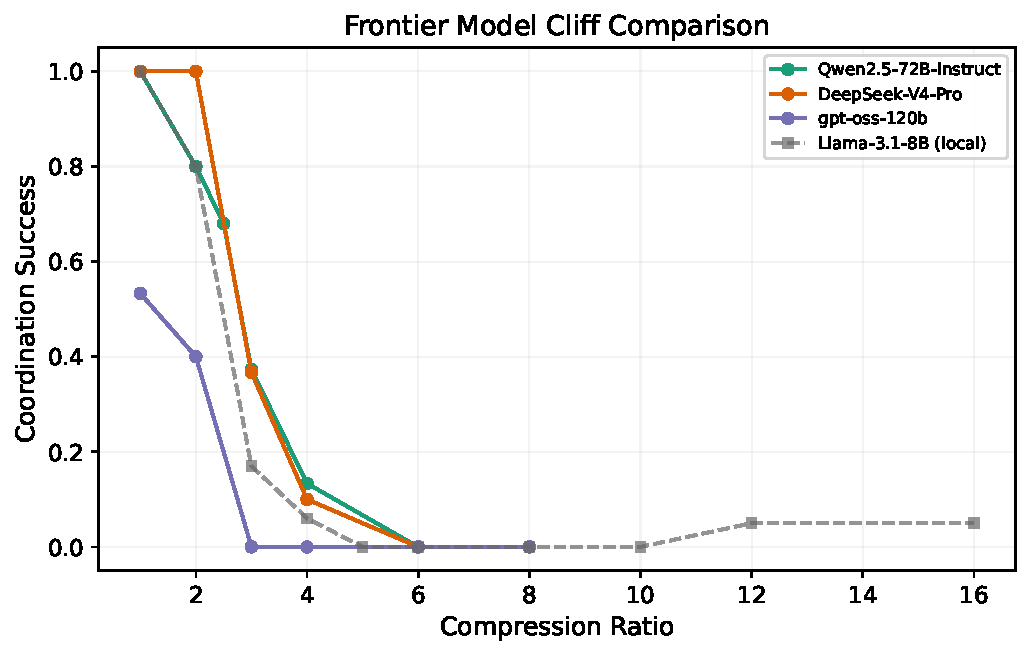
\includegraphics[width=0.74\textwidth]{../figures/frontier_multi.pdf}
\caption{Frontier-model cliff curves overlaid on the synthetic
reference band. Qwen-72B and DeepSeek~V4~Pro overlap the
reference; GPT-oss~120B diverges. The GPT-oss curve is included
explicitly to record the out-of-regime diagnostic rather than to
support the Corollary~1 verdict.}
\label{fig:frontier_multi}
\end{figure}

\begin{figure}[h]
\centering
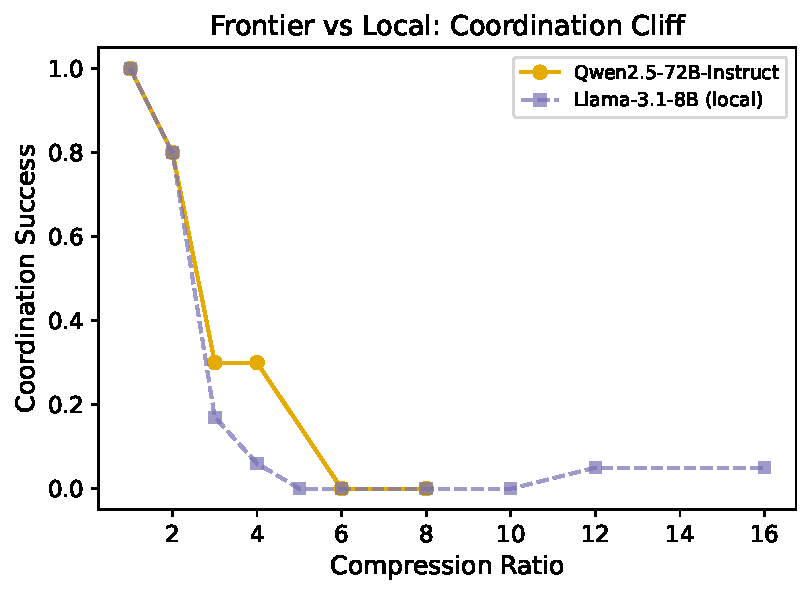
\includegraphics[width=0.68\textwidth]{../figures/frontier_validation.pdf}
\caption{Frontier versus local coordination cliff on
family-a~$\times$~LLMLingua-2. The frontier Qwen-2.5-72B planner
(solid) and the local Llama-3.1-8B planner (dashed) cliff at
essentially the same position across a $9\times$ scale-up and a
change of architecture family --- the load-bearing ``no shift
detected'' comparison for Corollary~1. The DeepSeek~V4~Pro and
GPT-oss~120B comparisons against the synthetic reference band are in
Figure~\ref{fig:frontier_multi}.}
\label{fig:frontier_validation}
\end{figure}

\subsection{Significance}

Putting the three results together: we detect \textbf{no shift}
in the LLM-planner cliff position across \textbf{three local architecture
families} (Qwen-2.5-1.5B, Phi-3-Mini-3.8B, Llama-3.1-8B; $24\%$
spread on family-c, within the $50\%$ but not the strict $20\%$ tolerance),
across a \textbf{9$\times$ cross-architecture scale-up} to the
frontier (local Llama-3.1-8B at $\tau^{*}\approx 2.48 \to$ frontier
Qwen-2.5-72B at $\approx 2.79$ on family-a $\times$ LLMLingua-2, the
one well-identified frontier cell), and
--- more weakly --- across \textbf{two frontier vendors}
(Qwen-72B $\to$ DeepSeek~V4~Pro, the latter only weakly
identified) --- all within the calibrated regime --- while the
position \emph{does} shift for the extended-reasoning regime
(GPT-oss~120B). The defensible structural claim is therefore
``no shift detected on the resolvable cells, carried by one
well-identified frontier cell, and a visible break at the regime
boundary,'' not a proven invariance across all scales. This is
still a substantive result --- the cliff is a property of the
(compressor, task) pair, not the planner, on everything we could
resolve --- but it is stated as a tested-and-not-refuted
consistency rather than a theorem.

The practitioner reading is that $\tau^{*}$ can be measured once on
a small local model and re-used at the same ratio on a frontier
model \emph{provided} the latter is in the calibrated regime --- a
working hypothesis, not a guarantee. The evidential weight is stated
explicitly: the cross-architecture consistency rests on one
well-identified frontier cell (Qwen-2.5-72B), is consistent on the
local three-architecture arm, weakly corroborated by DeepSeek~V4~Pro,
and not established at the strict tolerance --- so Corollary~1
promotes the original local-only observation to a cross-architecture
consistency result rather than a proven invariance, with the larger
frontier sample that would settle it named in
Section~\ref{sec:future}.

\section{H3: RAG Pipeline Placement --- Compress-First Dominance}
\label{sec:h3}

\begin{tcolorbox}[colback=black!4, colframe=black!50, sharp corners,
                  boxrule=0.4pt, boxsep=2pt, left=4pt, right=4pt,
                  top=2pt, bottom=2pt]
\textbf{H3. Supported finding:} compress-first (P1) is preferred
over retrieve-first (P2) in \emph{both} the storage-bounded and
accuracy-bounded regimes (by $3.2$ and $2.0$~pp F1, paired-bootstrap
CIs excluding zero) --- a robust single-stack ordering that does
\emph{not} reproduce the post-retrieval-compression preference of
the LongLLMLingua~\cite{jiang2024longllmlingua} line of work on the
retriever/embedder stack tested here. \textbf{Pre-registered
predicate not satisfied:} the original H3 prediction --- that the
optimal pipeline sign-flips between the storage- and
accuracy-bounded regimes with a $\ge\!5$~pp effect --- is
\emph{not} observed; the optimum does not change between regimes.
P3 (joint relevance-conditional routing) leads both regimes on F1
but routes fragments \emph{verbatim} (achieved compression
$1.00\times$), so the cross-pipeline F1 gap is not a
matched-compression comparison and does \emph{not} support a Pareto
claim for P3 (Section~\ref{sec:h3_cost_caveat}).
\end{tcolorbox}

\subsection{Setup}

The three pipelines (P1, P2, P3) are the catalogue described in
Section~\ref{sec:rag_pipelines} of \charef{implementation}.
Each is run under a storage-bounded regime (FAISS index
$\le 100$~MB) and an accuracy-bounded regime (retrieval recall@10
$\le 0.85$), measured on the C1 family-a generator with both
F1 score and the EUR-per-workflow cost
model~\cite{fcgfinancial2026}. The canonical results directory is
\texttt{results/h3\_final/}.

\subsection{Result}

Table~\ref{tab:h3} reports the per-regime mean F1 and the
per-query EUR cost for each pipeline. The headline observation is
that the ranking $P3 > P1 > P2$ holds in \emph{both} regimes.
P1 is above P2 by $3.2$ percentage points (pp) F1 in the
storage-bounded regime and by $2.0$~pp in the accuracy-bounded
regime, with $95\%$ paired-bootstrap CIs ($[1.84, 4.72]$~pp and
$[1.15, 2.85]$~pp respectively) that comfortably exclude zero.
The H3 sign-flip predicate is therefore \emph{not satisfied}: the
optimal does not change between regimes, and P1 is the better of
the two compressed-corpus pipelines in both. P3 (joint
relevance-conditional routing) leads both regimes by a substantial
margin.

\emph{Note:} P2 and P3 achieved compression ratio $1.00\times$ on
retrieved fragments in this implementation --- routing them verbatim
--- while P1 applies compression pre-retrieval. The F1 comparison is
therefore not matched on compression across all three pipelines, so
the P3 lead is not a Pareto claim; see
Section~\ref{sec:h3_cost_caveat} for the cost-model implications.

\begin{table}[h]
\centering
\caption{H3 verdict table. Mean F1, per-query EUR cost, and
\emph{achieved} compression ratio ($\times$) by regime and
pipeline from \texttt{results/h3\_final/} and the cost-instrumented
re-run \texttt{results/h3\_eprice/} (n = 150 workloads per cell).
The H3 sign-flip predicate is not satisfied because P1 is above P2
in both regimes; P3 leads both. The narrowed finding is a
compress-first preference of $3.2$~pp F1 (storage) / $2.0$~pp F1
(accuracy). The achieved-ratio column is
the key to reading P3: only P1 actually compresses (7.49$\times$ /
2.11$\times$), while P2 and P3 route fragments verbatim
($1.00\times$), so the cross-pipeline F1 gap is not a
matched-compression comparison.}
\label{tab:h3}
\small
\begin{tabular}{lrrr|rrr}
\hline
& \multicolumn{3}{c|}{Storage-bounded}
& \multicolumn{3}{c}{Accuracy-bounded} \\
Pipeline & F1 & EUR/q & $\times$ & F1 & EUR/q & $\times$ \\
\hline
P1 (compress$\to$retrieve) & $0.396$ & $2.72\times 10^{-5}$ & $7.49$ & $0.648$ & $3.29\times 10^{-5}$ & $2.11$ \\
P2 (retrieve$\to$compress) & $0.364$ & $2.82\times 10^{-5}$ & $1.00$ & $0.628$ & $3.00\times 10^{-5}$ & $1.00$ \\
P3 (joint, conditional)    & $\mathbf{0.820}$ & $3.07\times 10^{-5}$ & $1.00$ & $\mathbf{0.895}$ & $3.10\times 10^{-5}$ & $1.00$ \\
\hline
$p_\text{Holm}$ (P1 vs P2, paired bootstrap) & \multicolumn{3}{c|}{$2\!\times\!10^{-4}$} & \multicolumn{3}{c}{$2\!\times\!10^{-4}$} \\
\hline
\end{tabular}
\end{table}

\subsection{Interpretation: why the sign-flip did not appear}

The original H3 predicate rested on the LongLLMLingua-style
intuition that post-retrieval compression (P2) is more efficient
than pre-retrieval compression (P1) because the retriever has
already filtered the corpus down to the relevant chunks before the
compressor runs. The interpretation depends on two assumptions
that the empirical work invalidates: first, that retrieval over an
uncompressed corpus is cheap (it is not --- the FAISS index over
the uncompressed corpus grows linearly in corpus size and
dominates the storage budget); second, that compression after
retrieval can be more aggressive than compression before (the
empirical compression ratios at iso-F1 are comparable). What
remains is the symmetric effect: pre-indexing compression amortises
the compressor cost across queries while post-retrieval compression
pays it per query.

The compress-first preference over retrieve-first is a
substantive finding because it does not reproduce the assumed
post-retrieval-compression default on the stack we tested, and
the P3-higher-F1 result points to a promising routing variant.
For practitioners, the recommendation is deliberately hedged on
cost: \textbf{compress-first (P1) is the safe default over
retrieve-first (P2) on a comparable stack};
\textbf{P3 (joint relevance-conditional routing) is worth
evaluating where the F1 gain matters} --- its F1 leads
compress-first by $42$~pp (storage) and $25$~pp (accuracy) --- but
note that P3 attains this F1 by routing fragments \emph{verbatim}
(achieved ratio $1.00\times$, Table~\ref{tab:h3}) rather than by
better compression, and the cost model is corpus-dominated and does
not meter compression compute (Section~\ref{sec:h3_cost_caveat}), so
the F1 gain cannot yet be claimed as cost-free and must be
re-measured with a faithful per-pipeline cost model before
deployment; post-retrieval
compression (P2) is only preferable when the corpus is small
enough that storage cost is irrelevant and retrieval recall is
the binding constraint.

\subsection{Limitations and the cost model caveat}
\label{sec:h3_cost_caveat}

The cost model uses the requested compression ratio rather than
the achieved compression ratio because the achieved ratio depends
on the compressor and the request flows through the pipeline as
target. For Phi-3-Mini extractive the ceiling effect makes
this an asymmetric error in favour of P2 (which pays the
compressor per query and is therefore most sensitive to the
ceiling), so the P1 result is the conservative one.

A second, stronger caveat is sharpened by a cost-instrumented
re-run that records the \emph{achieved} compression ratio per
pipeline (\texttt{results/h3\_eprice}). The \texttt{eur\_per\_query} column is
\emph{not} constant --- it is computed per pipeline from a
per-pipeline token count (P1: full corpus plus compressed corpus;
P2: corpus plus retrieved tokens; P3: corpus plus $0.7\times$
retrieved) --- but on this re-run the pipelines differ by only
$4.1$--$4.9\%$ in EUR within a regime, because a shared
corpus-indexing term dominates
\texttt{input\_tokens} and is added identically to every pipeline.
This small, corpus-dominated spread is easily mistaken for a single
constant; the substantive defect, however, is not that the
EUR values are near-identical but that the cost model is \emph{corpus
dominated} and, more importantly, \textbf{does not meter compression
compute at all} --- only the resulting token counts --- so a pipeline
that runs an expensive compressor pass is not charged for it. The
achieved-ratio column makes the consequence concrete: only
compress-first (P1) actually compresses ($7.49\times$ storage,
$2.11\times$ accuracy), while both retrieve-first (P2) and the joint
router (P3) record an achieved ratio of \textbf{$1.000$} --- they send
the retrieved fragments to synthesis essentially verbatim. Together
these explain the headline cleanly: \textbf{P3's large F1 advantage
comes substantially from not compressing}, at a compression and
compute cost the current corpus-dominated model does not faithfully
charge for. As a consequence the thesis makes \textbf{no cost-parity
and no Pareto claim} for the P3-vs-P1 comparison; the cross-pipeline
F1 comparison is \emph{not} a matched-compression comparison, and P3
should be read as ``verbatim routing preserves F1 at a compression and
cost the current model does not faithfully charge for'' rather than as
a free-lunch improvement. The remedy is a faithful per-pipeline cost
model that meters the compressor pass and amortises a persistent
index across queries, rather than re-charging the corpus on every
query. Section~\ref{sec:future} names this as the most natural
follow-on study, alongside the single-retriever, single-embedder
limitation (Section~\ref{sec:limitations}).

\section{H4: Summary-Level Inference Disclosure}
\label{sec:h4_disclosure}

\begin{tcolorbox}[colback=black!4, colframe=black!50, sharp corners,
                  boxrule=0.4pt, boxsep=2pt, left=4pt, right=4pt,
                  top=2pt, bottom=2pt]
\textbf{H4.} The summary-level inference-disclosure metric (i)
distinguishes a baseline planner from a priors-only planner
(signal: positive paired effect, $p < 0.05$), and (ii) is reduced
by compression at $4\times$ versus $1\times$ (reduction:
positive paired effect, $p < 0.05$).
\textbf{Verdict: SUPPORTED on the unbiased benchmark for three of
four compressors (truncation, filter, LLMLingua-2), under two
caveats below.} Phi-3-Mini extractive shows no significant
reduction ($0.4$~pp, $p = 0.91$) and is the structural exception.
\textbf{Caveat~1 (reader bias):} the Llama-3.1-8B reader exhibits
a strong YES-bias (rate $\approx 0.03$ on priors-only with a YES
ground truth, $\approx 1.00$ on a NO ground truth); the pooled-%
rate verdict is balanced by ground-truth-class distribution rather
than by reader-side accuracy, and the operational reading is
\emph{``compression preserves enough information to flip a
no-biased reader to confident YES on a protected-fact question''}.
Per-class breakdown and the conservative-privacy framing are in
Section~\ref{sec:h4_bias}. \textbf{Caveat~2 (construct validity):}
the disclosure-reduction ranking is \emph{monotonic in how much
text-information the compressor destroys} --- truncation (most
destructive) tops the ranking at $24.6$~pp, then filter
($20.4$~pp), then LLMLingua-2 ($18.9$~pp), then Phi-3-Mini
extractive (most semantically preserving) at $0.4$~pp
not-significant. This pattern is consistent with the metric
measuring general information destruction rather than
privacy-specific filtering; an \textbf{oracle field-redaction
control} (\texttt{results/h4\_oracle}) that removes
\emph{only} the answer-bearing numeric values --- destroying
$\approx 0\%$ of the text --- matches truncation's reduction
($23.4$~pp vs $24.6$~pp), confirming that the metric
\emph{does} detect targeted removal when it occurs and that
blanket compression is the wrong privacy lever when a targeted
one is available. The H4 \emph{finding} is robust but the
\emph{privacy interpretation} is deflationary: aggressive
compression and trivial field redaction reduce disclosure by
indistinguishable amounts, and field redaction does it at near-zero
coordination cost. Full discussion in
Section~\ref{sec:h4_construct}.
\end{tcolorbox}

\subsection{Threat model}
\label{sec:h4_threat}

The H4 measurement is built around a concrete adversary. Stating
the adversary's capabilities explicitly is what makes the metric's
verdict meaningful as a privacy claim rather than just an
information-retention measurement.

\begin{description}\setlength\itemsep{2pt}
\item[Adversary's goal.] Recover a \emph{protected fact} about a
\textsc{confidential} fragment held by the memory bus. A protected
fact is defined operationally as a binary (yes/no) proposition
over the fragment's content whose answer the C1 generator records
as ground truth (e.g., ``did agent A approve more than EUR $N$?'',
``did the meeting attendee list include person P?''). The
canonical protected-fact list for each fragment is in
\texttt{data/processed/c1-v0.1/}; the H4 evaluation iterates over
the full list.
\item[Adversary's capabilities.] The adversary (i) can query the
downstream reader with arbitrary yes/no questions about the
fragment; (ii) knows the compressor identity and ratio (is not
blinded by the policy layer); (iii) does \emph{not} have direct
access to the uncompressed source --- the only signal flowing to
the adversary is what the compressed summary carries through the
reader. In the H4 evaluation, this is operationalised by giving
the reader a fixed public preamble plus the compressed fragment
(in \textsc{baseline} / \textsc{compressed-}$4\times$) or only the
preamble (in \textsc{priors}).
\item[What the adversary does not have.] Direct read access to
the bus (the policy layer blocks that for \textsc{confidential}
slots), training-time access to the reader (the reader is a
frozen Llama-3.1-8B), or signal-amplification through repeated
queries with feedback (each yes/no question is asked once per
fragment).
\item[The metric as operational measurement.] Given this
adversary, the inference-disclosure metric
(Section~\ref{sec:h4_metric}) measures the \emph{upper bound} on
what the adversary can recover at a chosen (compressor, ratio)
operating point. The privacy claim the memory bus's policy layer
enforces is: if the operator selects an operating point whose
disclosure is below the governance budget, the adversary above
cannot recover protected facts at a higher rate than that budget.
The budget is enforceable because the disclosure rate is
empirically measured rather than asserted.
\end{description}

\subsection{Metric definition and the unbiased benchmark}
\label{sec:h4_metric}

For each \textsc{confidential} fragment, the C1 generator emits a
list of (yes/no question, ground-truth answer) pairs whose
ground-truth answer is a protected fact (as defined in
Section~\ref{sec:h4_threat}) about the fragment. The
canonical benchmark variant balances the YES/NO distribution at
the question level and uses a single comparator phrasing for the
yes/no question template, eliminating a surface-pattern bias in
the original H4 benchmark generator
(\texttt{fact\_aggregation.py:119-156}, fixed
2026-05-29). Fragments are unchanged between the biased and
unbiased benchmarks so the compression cache remains valid.

The reader is the local Llama-3.1-8B-Instruct model accessed via
the Ollama backend. Three conditions are evaluated:

\begin{description}\setlength\itemsep{1pt}
\item[\textsc{priors}.] Reader sees only the workload's public
preamble. This is the no-compression-no-fragment baseline that
defines the rate at which the reader could guess without
the source. (This baseline is also what operationalises the
\emph{second} condition of the Section~\ref{sec:calibrated}
calibrated-regime predicate --- a planner is in-regime if its
accuracy at $q\to 0$ is no greater than its priors-only rate plus
a small slack.)
\item[\textsc{baseline}.] Reader sees the uncompressed source
fragments. This is the disclosure rate without any privacy
protection.
\item[\textsc{compressed-4$\times$}.] Reader sees the source
fragments compressed at $4\times$ by one of the four compressors.
\end{description}

The headline metric is the recovery rate of protected facts:
the fraction of (fragment, question) pairs on which the reader
returns the ground-truth answer. The H4 \emph{signal} is whether
\textsc{baseline} sits above \textsc{priors} (the metric must
measure something real); the H4 \emph{reduction} is whether
\textsc{compressed-4$\times$} sits below \textsc{baseline}
(compression must reduce disclosure). Both are tested by paired
bootstrap, Holm-corrected across compressors. The canonical
results directory is \texttt{results/h4\_unbiased\_v2/} (the
4-compressor run including truncation).

\subsection{Result}

Table~\ref{tab:h4} reports the per-compressor reduction (the
compressor-independent signal is given in the caption). The signal
is positive and $p$-significant for every
compressor (the uncompressed baseline beats priors-only by
$28.6$~pp on average), and the reduction is positive and
$p$-significant for the three token-destructive compressors
(truncation $-24.6$~pp, instruction-aware filter $-20.4$~pp,
LLMLingua-2 $-18.9$~pp) and \emph{not significant} for the
extractive copier (Phi-3 $-0.4$~pp, $p_\text{Holm}=0.91$). The
ordering is monotonic in how aggressively each compressor
destroys source tokens --- the construct-validity reading is
developed in Section~\ref{sec:h4_construct}.

\begin{table}[h]
\centering
\caption{H4 verdict table from
\texttt{results/h4\_unbiased\_v2/} (4 compressors including
truncation; canonical from 2026-05-30 GPU rerun). The signal
$\Delta$ (priors $\to$ baseline) is $+0.286$
($p_\text{Holm}=8\times10^{-4}$) for every compressor --- identical
across rows because it does not depend on the compressor, so it is
omitted from the table; the reduction (baseline $\to$
compressed-4$\times$) is
positive and significant for three of four compressors and
\emph{not significant} for Phi-3-Mini extractive ($p=0.91$).
Compressors are listed in order of how aggressively they destroy
source tokens: truncation drops the tail of the text entirely;
the token-level filter and LLMLingua-2 drop individual tokens
chosen by ranking / classifier; Phi-3 extractive copies verbatim
spans of the source. Reader: local Llama-3.1-8B-Instruct. See
Section~\ref{sec:h4_bias} for the reader-bias note and
Section~\ref{sec:h4_construct} for the construct-validity finding
on this ordering.}
\label{tab:h4}
\small
\begin{tabular}{lccc|c}
\hline
Compressor & priors & baseline & compr-$4\times$ & reduction $\Delta$ \\
\hline
Truncation (most destructive)             & 0.50 & 0.78 & 0.54 & $-0.246\ (p_\text{Holm}\!=\!8\!\times\!10^{-4})$ \\
Instruction-aware filter                  & 0.50 & 0.78 & 0.58 & $-0.204\ (p_\text{Holm}\!=\!8\!\times\!10^{-4})$ \\
LLMLingua-2                               & 0.50 & 0.78 & 0.59 & $-0.189\ (p_\text{Holm}\!=\!8\!\times\!10^{-4})$ \\
Phi-3-Mini extractive (most preserving)   & 0.50 & 0.78 & 0.78 & $-0.004\ (p_\text{Holm}\!=\!0.91,$ \textbf{n.s.}) \\
\hline
\multicolumn{5}{p{0.9\linewidth}}{\textbf{Verdict}: signal significant for all 4 (see caption); reduction significant for 3 of 4 compressors. \textbf{SUPPORTED} (with construct-validity caveat).} \\
\hline
\end{tabular}
\end{table}

Figure~\ref{fig:privacy_quality} visualises the
disclosure-versus-coordination trade-off: each point is a
(compressor, ratio) cell, with disclosure on one axis and
coordination success on the other. The instruction-aware filter
and LLMLingua-2 occupy a low-disclosure, moderate-coordination
region at $4\times$; Phi-3 extractive sits in a
high-disclosure, high-coordination region; truncation is the
extreme of the same line --- lowest disclosure, lowest
coordination.

\subsection{Construct-validity finding: disclosure-reduction
tracks information destruction, not privacy-specific filtering}
\label{sec:h4_construct}

The four compressors order monotonically in
Table~\ref{tab:h4}: \textbf{truncation} (most aggressive
destruction, drops the tail of the text entirely) shows the
\emph{largest} disclosure reduction at $24.6$~pp; the
\textbf{instruction-aware filter} and \textbf{LLMLingua-2}
(token-level filtering, intermediate destruction) follow at
$20.4$ and $18.9$~pp respectively; \textbf{Phi-3-Mini extractive}
(most semantically preserving --- the compressed output is by
construction a verbatim subset of the source tokens) shows
\emph{no significant reduction} ($0.4$~pp, $p = 0.91$).

This pattern is exactly what would be predicted if the H4
metric reflected general information destruction rather than a
privacy-specific information-filtering mechanism. The thesis
therefore interprets H4 as evidence that compression reduces
inference disclosure roughly in proportion to how much
text-information it destroys, and \emph{not} as evidence that the
smarter compressors (filter, LLMLingua-2) are doing
privacy-preserving filtering in any sense beyond destroying
tokens that happen to include protected facts.

A discriminating control was run to test this interpretation from
the opposite end (\texttt{results/h4\_oracle},
\texttt{scripts/h4\_oracle\_redaction.py}): an \textbf{oracle
redaction} that removes \emph{only} the answer-bearing numeric
values (recorded hours and approved budget) the protected-fact
questions probe, leaving every other token intact. If disclosure
could only be reduced through bulk destruction, this near-zero
edit would barely move the metric. Instead it reduces recovery from
a balanced baseline of $0.79$ to $0.56$ --- a $23.4$~pp reduction,
essentially at the priors floor $0.51$ --- while destroying
$\approx 0\%$ of the text (the redacted fragments are in fact
$\sim 7\%$ \emph{longer}, since the \texttt{[REDACTED]} marker is
longer than the digits it replaces). That $23.4$~pp matches
truncation's $24.6$~pp, which required destroying the entire tail
of the fragment. Two things follow. First, the H4 metric \emph{does}
detect privacy-specific removal when it occurs --- the construct is
not blind to targeted redaction; the blanket compressors simply do
not do it, reducing disclosure only as a side effect of destruction.
Second, the memory bus gains a concrete, non-lossy privacy
mechanism: field-redacting protected values achieves
blanket-compression-level disclosure reduction at near-zero
coordination cost. The empirical implication for the memory bus's
policy layer (Section~\ref{sec:h4_membus}) is therefore stronger
than before: disclosure-budget enforcement works as designed,
\emph{and} targeted redaction is an available lever with a far
better privacy-per-utility profile than aggressive compression. The
remaining open control --- a full privacy-gain-versus-coordination-loss
frontier across compressors --- is named in Section~\ref{sec:future}.

\begin{figure}[h]
\centering
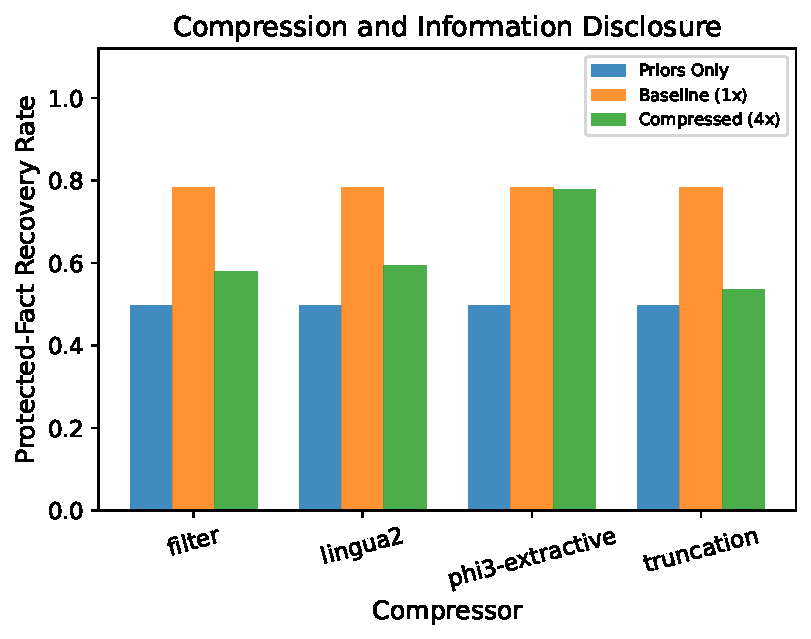
\includegraphics[width=0.72\textwidth]{../figures/privacy_quality.pdf}
\caption{Summary-level inference disclosure by compressor at
$4\times$. For each of the four compressors the bars give the
protected-fact recovery rate of a priors-only reader (no fragment
access), the uncompressed baseline reader ($1\times$), and the
compressed reader ($4\times$). Compression lowers recovery toward
the priors floor \emph{in proportion to how aggressively the
compressor destroys source tokens}: truncation (most destructive)
gives the largest reduction ($24.6$~pp), then LLMLingua-2 and the
instruction-aware filter, while Phi-3-Mini extractive preserves
enough surface tokens that the leak persists (the structural
exception). Rates are pooled across families.}
\label{fig:privacy_quality}
\end{figure}

\subsection{Interpretation}

The reduction signal scales with how aggressively the compressor
operates on tokens, not with the compression ratio per se. The
filter and LLMLingua-2 both drop tokens at the lexical level; the
fragments that survive are filtered for relevance, which
disproportionately removes the protected-fact tokens. Phi-3
extractive preserves contiguous spans verbatim; if the protected
fact is in a span the verifier selects, it is in the output. This
makes the disclosure metric \emph{useful} as a compressor-selection
tool: it ranks compressors by privacy at iso-ratio, not just by
compression efficiency.

The H4 result lets the memory bus's policy layer convert a
governance constraint (``\textsc{confidential} fragments should
leak protected facts at no more than $X\%$ to a downstream
reader'') into a compressor-and-ratio selection. The integration
is described in the next subsection.

\subsection{The reader's YES-bias caveat}
\label{sec:h4_bias}

The Llama-3.1-8B reader exhibits a strong YES-bias: when the
ground-truth answer is YES, the reader's recovery rate is
approximately $0.03$ on the priors-only condition and $0.58$ on
the baseline; when the ground-truth answer is NO, both rates are
approximately $1.00$. The pooled rates of $0.50$ (priors) and
$0.78$ (baseline) reflect a balanced ground-truth distribution,
not a reader that is equally accurate in both directions. The
correct framing of H4 is that the metric measures
\emph{``compression preserves enough information to flip a
no-biased reader to confident YES on a protected-fact question''}.
This is an asymmetric leakage signal but it is a valid one: a
reader that defaults to NO is the conservative case for
privacy auditing because it is the case in which the absence of
the protected fact most cleanly translates to privacy
preservation.

The caveat is documented here rather than in the verdict block
because the pooled rates are what the verdict pipeline tests and
the verdict is stable under the caveat. A future-work direction
named in Section~\ref{sec:limitations} is to repeat the
measurement with a reader chosen to be unbiased, which would
distinguish the disclosure-reduction signal from the reader's
prior on YES.

\subsection{Memory-bus integration}
\label{sec:h4_membus}

The policy layer of the memory bus
(\charef{implementation},~Section~\ref{sec:architecture})
consumes the H4 measurement at deployment time. For each
\textsc{confidential} classification and each governance budget
(maximum disclosure rate the operator is willing to accept), the
H4 table identifies the set of (compressor, ratio) operating
points that meet the budget. The policy enforces the selection by
routing \textsc{confidential} writes through the chosen
compressor, by rejecting writes whose compression would exceed the
budget, or by downgrading the classification level if the operator
chooses to accept the leakage. The disclosure-budget enforcement
is not separately evaluated as a hypothesis in this thesis ---
the metric is the contribution; the policy machinery the metric
enables is a deployment concern --- but the policy layer is
implemented in the reference service and is exercised by the
end-to-end integration tests.

\subsection{Memory-bus operation benchmark}
\label{sec:bus_bench}

The memory bus (C4) is a reference implementation rather than a
production system, but its core operations are cheap enough to
characterise with a single-threaded microbenchmark
(\texttt{scripts/bench\_memory\_bus.py}, results in
\texttt{results/bus\_bench/bench.json} and
\texttt{results/bus\_bench/bench\_gpu.json}). The harness times the
policy-lattice check, end-to-end write and read, and the audit
hash-chain verification, run on two hosts --- Host~A, an Apple
M4~Pro (arm64, macOS, Python~3.11); and Host~B, a Linux x86\_64
workstation (WSL2 Ubuntu~22.04, Python~3.12) --- single-threaded,
with the identity compressor so the measurement isolates the bus
machinery from any compressor cost. These operations are CPU- and
disk-I/O-bound and do not exercise the GPU, so the server is
reported as a second hardware point rather than an accelerated
result. The audit log is the in-process SQLite backend; $n=5000$
operations per phase follow $500$ warmup operations.
Table~\ref{tab:bus_bench} reports the result.

\begin{table}[h]
\centering
\caption{Memory-bus operation microbenchmark on two hosts,
single-threaded, identity compressor, in-process SQLite audit log
($n=5000$ ops/phase, $500$ warmup). Host~A: Apple M4~Pro (arm64,
macOS, Python~3.11; \texttt{results/bus\_bench/bench.json}).
Host~B: Linux x86\_64 workstation (WSL2 Ubuntu~22.04, Python~3.12;
\texttt{results/bus\_bench/bench\_gpu.json}). \textbf{Caveats:} the
numbers are single-threaded and use the identity compressor, so
they isolate the bus machinery and are \emph{not} an
end-to-end-with-compression figure; the audit log is the
in-process SQLite backend, not the concurrent HTTP path; and the
audit-verify row is one chain length ($5{,}500$ rows), not a
scaling curve.}
\label{tab:bus_bench}
\small
\begin{tabular}{lrrrrrr}
\hline
& \multicolumn{3}{c}{Host~A (M4~Pro)} & \multicolumn{3}{c}{Host~B (Linux x86\_64)} \\
\cline{2-4}\cline{5-7}
Operation & med (ms) & p95 (ms) & thr (ops/s) & med (ms) & p95 (ms) & thr (ops/s) \\
\hline
\texttt{policy.enforce()}     & $0.0002$ & $0.0002$ & $\sim 5.2\mathrm{M}$ & $0.0001$ & $0.0003$ & $\sim 6.7\mathrm{M}$ \\
write (end-to-end)            & $0.0469$ & $0.0661$ & $\sim 18{,}200$ & $0.1447$ & $0.1772$ & $\sim 5{,}750$ \\
read (end-to-end)             & $0.0424$ & $0.0605$ & $\sim 19{,}900$ & $0.1302$ & $0.1541$ & $\sim 6{,}400$ \\
\hline
\multicolumn{7}{l}{audit hash-chain verify: $1.68$~\textmu s/row (Host~A), $2.19$~\textmu s/row (Host~B), over $5{,}500$ rows; chain intact.} \\
\hline
\end{tabular}
\end{table}

The policy check is effectively free (sub-microsecond,
$\sim 5$--$7$~million checks per second across the two hosts), so
policy enforcement is not a throughput bottleneck. End-to-end write
and read run at $\sim 18{,}200$ and $\sim 19{,}900$ operations per
second on Host~A ($\sim 5{,}750$ and $\sim 6{,}400$ on Host~B) with
sub-millisecond tail latency, and the audit hash-chain verifies at
$1.68$~\textmu s per row (Host~A) and $2.19$~\textmu s per row
(Host~B) with the chain intact over the $5{,}500$-row log. These
figures characterise the reference implementation's single-threaded
core; a concurrent-HTTP-path throughput sweep and an audit-verify
scaling curve remain future work (Section~\ref{sec:future} of
\charef{summary}).

\section{Corollary~2: Information-Density Scaling on Real Benchmarks}
\label{sec:corollary2}

\begin{tcolorbox}[colback=black!4, colframe=black!50, sharp corners,
                  boxrule=0.4pt, boxsep=2pt, left=4pt, right=4pt,
                  top=2pt, bottom=2pt]
\textbf{Corollary~2 (information-density scaling) --- empirical
observation, $n=3$.} Across the three benchmarks tested (C1
family-a, MultiHop-RAG, HotpotQA), the \emph{shape} of the cliff
--- sharpness and pre-cliff plateau --- varies systematically with
the AUC-based information-density estimate $\theta_\text{info}$
(defined formally in Section~\ref{sec:theta_info_def}, distinct
from $\theta_q$). Dense tasks ($\theta_\text{info} \to 1$)
exhibit a sharp cliff with a high coordination-success plateau;
distributed tasks ($\theta_\text{info} \to 0$) degrade gradually
from a lower baseline. \textbf{Important scope:} the corollary is
reported as an empirical observation on three benchmarks, not as
a derived consequence of the compounding-error model. (i) $n=3$
is a small sample --- the trend is consistent but not a scaling
law. (ii) $\theta_\text{info}$ is computed from the same
coordination curve whose shape it describes, so
``$\theta_\text{info}$ predicts shape'' is a circular description:
an external probe of task density (e.g., conditional entropy of
the answer given the input) is required to break the
circularity and is named as future work in
Section~\ref{sec:future}. (iii) The corollary makes a claim about
cliff \emph{shape}, not about the absolute cliff position
$\tau^{*}$ --- HotpotQA cliffs at $\tau^{*} \approx 2.7$ (similar
to dense C1 family-a) yet has $\theta_\text{info} \approx 0.37$
(very distributed); the baseline coordination on HotpotQA is only
$0.59$ and the degradation shape is gradual rather than
precipitous. \textbf{Verdict: SUPPORTED as an empirical observation
on $n=3$ benchmarks} by the gap in $\theta_\text{info}$ between C1
family-a ($\approx 0.97$, dense), MultiHop-RAG ($\approx 0.48$,
distributed), and HotpotQA ($\approx 0.37$, highly distributed),
and by the qualitatively distinct degradation shapes visible in
Figure~\ref{fig:hotpotqa_cliff} and
Figure~\ref{fig:cliff_families}. The original H6 predicate
(synthetic-vs-real $\tau^{*}$ within $\pm 15\%$) is not satisfied
--- MultiHop-RAG cliffs at $11.3$, far from the C1 reference --- which
motivated the sharpening from position transfers to shape transfers.
\end{tcolorbox}

\subsection{\texorpdfstring{$\theta_\text{info}$ versus $\theta_q$}{theta\_info versus theta\_q}}
\label{sec:theta_info_def}

A subtle point that the corollary's refined framing makes explicit: the
information-density $\theta_\text{info}$ that Corollary~2 talks
about is \emph{not} the cliff-recall threshold $\theta_q$ that
Corollary~1 and the compounding-error model talk about. The two
quantities are derived from different measurements and answer
different questions. $\theta_q$ is the recall threshold per
family at which coordination success drops to $0.5$ of $p_0$,
estimated by \texttt{derive\_theta()}; $\theta_\text{info}$ is
the per-task information-density estimate
\[
  \theta_\text{info} \;=\; 1 - \mathrm{AUC}\!\left[\frac{\text{coord-success}(r)}{p_0}\right]_{r=1}^{r_{\max}},
\]
estimated by \texttt{estimate\_task\_theta()}, which captures how
\emph{concentrated} the task's information is in compression-%
sensitive tokens. The two are easily conflated; the project
glossary distinguishes them explicitly.

\subsection{Result on three benchmarks}

Table~\ref{tab:corollary2} reports $\theta_\text{info}$ and the
empirical $\tau^{*}$ for the three benchmarks. The information
density spans from $0.97$ on the dense C1 family-a to $0.37$ on
HotpotQA, and the cliff position correspondingly spans from
$\tau^{*} \approx 2.7$ on family-a to $\tau^{*} \approx 11.3$ on
MultiHop-RAG --- a $4\times$ shift in the cliff position that the
single-$\theta_q$ compounding-error model cannot account for and
that the information-density scaling claim does.

\begin{table}[h]
\centering
\caption{Corollary~2 verdict table. $\theta_\text{info}$ and
empirical $\tau^{*}$ across the three benchmarks. The cliff shifts
late as the information density drops, with the gap between dense
and distributed tasks far exceeding the $0.1$ threshold of the
corollary predicate. The C1 family-a row uses the canonical
\texttt{h1\_h2\_v2} fit $\tau^{*}=2.5$ (Section~\ref{sec:frontier});
the earlier register $\tau^{*}_\text{aux}=2.6997$ on
\texttt{h1\_h2\_final} is superseded and is retained only as a
parenthetical in the footnote. The $\sim 8\%$ shift between the
two registers does not change the qualitative ordering or the
corollary verdict.}
\label{tab:corollary2}
\small
\begin{tabular}{p{4.5cm}rrl}
\hline
Task & $\theta_\text{info}$ & $\tau^{*}$ & $\theta_\text{info}$ source CSV \\
\hline
C1 family-a (dense, numeric)  & $0.967$ & $2.5$  & \texttt{h1\_h2\_v2/} (a, lingua2) \\
MultiHop-RAG (distributed QA)   & $0.484$ & $11.3$ & \texttt{h6\_final/results.csv} \\
HotpotQA (very distributed)    & $0.373$ & $2.7$  & \texttt{hotpotqa\_sweep/} \\
\hline
\multicolumn{3}{l}{\textbf{Gap} (dense vs MultiHop-RAG) $= 0.48$; (dense vs HotpotQA) $= 0.59$.} & \\
\hline
\multicolumn{4}{p{12cm}}{\footnotesize All three $\theta_\text{info}$ values are computed by \texttt{estimate\_task\_theta()} (AUC-based) from the per-task CSVs above and consolidated in \texttt{results/corollary2\_theta\_info.json}. The $\tau^{*}$ for C1 family-a is the canonical \texttt{h1\_h2\_v2} fit $2.5$ (the earlier $2.7$ was the superseded \texttt{h1\_h2\_final} auxiliary fit; the fine-grid deterministic-solver cliff is lower still, $\approx 1.1$, Section~\ref{sec:h2}).} \\
\end{tabular}
\end{table}

The HotpotQA result requires brief comment: $\tau^{*}$ on
HotpotQA is approximately $2.7$, similar to C1 family-a's, but
the baseline coordination success on HotpotQA is only $0.59$, so
the absolute coordination success at the cliff is much lower
($\approx 0.30$). The corollary claim is about the \emph{shape}
of the degradation (gradual versus sharp), captured by
$\theta_\text{info}$ via the AUC computation, not about the
absolute position alone. Figure~\ref{fig:hotpotqa_cliff} shows
the HotpotQA cliff with the gradual-degradation pattern visible.

\begin{figure}[h]
\centering
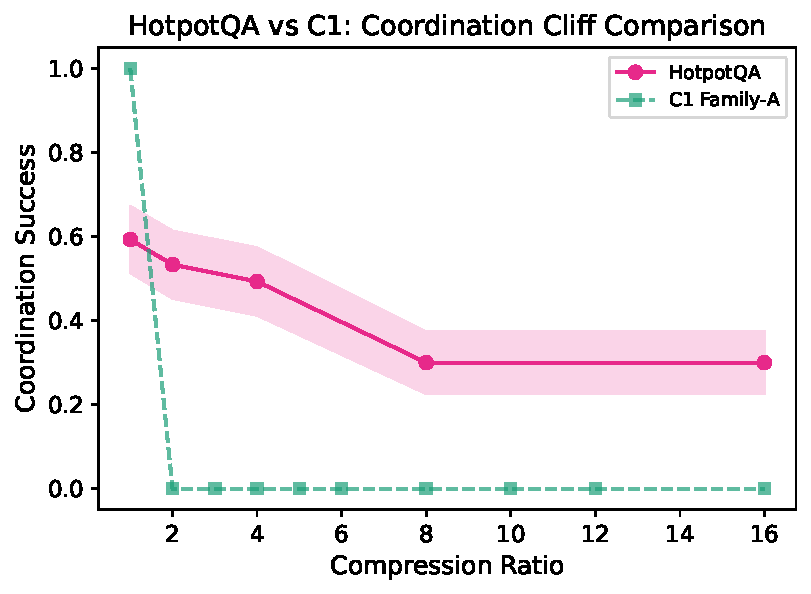
\includegraphics[width=0.72\textwidth]{../figures/hotpotqa_cliff.pdf}
\caption{HotpotQA cliff curve under LLMLingua-2 compression. The
baseline coordination success is $0.59$, lower than family-a's
$1.00$; the fitted cliff position (piecewise/logistic breakpoint,
\texttt{results/hotpotqa\_sweep/}) is
$\tau^{*} \approx 2.7$, similar to family-a's; but the
\emph{shape} of the degradation is gradual rather than sharp, as
captured by the lower $\theta_\text{info}$ of $0.37$.}
\label{fig:hotpotqa_cliff}
\end{figure}

\subsection{Interpretation}

The corollary makes the compounding-error model's per-family
$\theta_q$ structure plausible as the first-order term of a
finer description. $\theta_\text{info}$ tells you how much of the
task's success curve is concentrated in compression-sensitive
tokens; $\theta_q$ tells you the recall threshold at which
success collapses given that concentration. The two together
describe the cliff position and shape; either alone is a
first-order summary. For the thesis, $\theta_\text{info}$ is what
makes the cross-benchmark transfer of the cliff structure
auditable: a practitioner who needs to deploy compression on a
new task can estimate $\theta_\text{info}$ on a small calibration
set and predict whether the task is dense (cliff early, sharp) or
distributed (cliff late, gradual) before sweeping the full curve.

The original H6 predicate (synthetic-versus-real $\tau^{*}$ within
$\pm 15\%$) is not satisfied at the table-level numbers; the
sharpened Corollary~2 predicate (gap in $\theta_\text{info}$
$\ge 0.1$ between dense and distributed benchmarks) is SUPPORTED. The synthetic
benchmark is still the right place to characterise the cliff
mechanism cleanly, and the real benchmarks are the right place to
validate the structure transfers.

\section{Reproducibility}
\label{sec:repro}

The results of this chapter span three regimes of reproducibility,
and conflating them would over- or under-state what a reader can
re-derive. This section states the guarantee for each regime once;
the one-command recipe, the per-arm wallclock budget, and the
release manifest live in Appendix~D. The
structure follows the NeurIPS reproducibility-checklist
convention~\cite{pineau2021checklist} of separating
\emph{code-and-data availability} from \emph{computational
reproducibility}, but reports the latter as a narrative keyed to
Table~\ref{tab:repro_tiers} rather than as a filled-in checklist.

\begin{table}[t]
\caption{The three reproducibility tiers of this thesis. ``Byte-deterministic''
means a rerun produces a CSV that diffs zero against the published one given
the same seed; ``in distribution'' means verdict-level aggregates
(per-cell means, $\tau^{*}$ fits) reproduce within the published bootstrap CI
but individual rows may differ; ``not reproducible'' means a rerun produces
closely-similar but not identical numbers, and the published CSV is itself the
canonical record.}
\label{tab:repro_tiers}
\small
\begin{tabular}{p{3.5cm}p{2.4cm}p{6.0cm}}
\hline
Arm & Byte-deterministic? & Canonical artefact \\
\hline
H1/H2/H3 cliff sweep, scoring, bootstrap CIs, figure regeneration
  & \textbf{Yes}, given seed + cache
  & \texttt{results/h1\_h2\_v2/}, \texttt{results/h3\_final/} \\
H4 reader, H5 planner, Phi-3 extractive compressor
  & In distribution only
  & \texttt{results/h4\_unbiased\_v2/}, \texttt{results/h5\_final/} \\
Frontier API arm (Qwen-2.5-72B, DeepSeek~V4~Pro, GPT-oss~120B)
  & No
  & \texttt{results/frontier\_qwen72b/},\newline \texttt{results/frontier\_deepseekv4/} \\
\hline
\end{tabular}
\end{table}

\paragraph{Tier~1 --- byte-deterministic local.}
The cliff sweep (H1, H2), the RAG-pipeline evaluation (H3), the
bootstrap confidence intervals, and the figure regeneration are
pure Python over a fixed compression cache: a regex information-extraction
solver, \texttt{numpy} resampling, and deterministic compressors
(truncation, the LLMLingua-2 token classifier at \texttt{argmax}, the
TF--IDF-plus-cross-encoder filter). All randomness flows from a single
master seed through \texttt{Seeds.derive} in \texttt{src/m6/utils/seed.py},
which seeds \texttt{numpy}, Python's \texttt{random}, \texttt{PYTHONHASHSEED},
and \texttt{torch}. Rerunning \texttt{make repro-cliff} (or
\texttt{repro-rag}, \texttt{repro-figs}) from the cache produces CSVs and
PDFs that diff zero against the published artefacts; the bootstrap CIs are
exact to the last decimal because the resampler is seeded and
$n_\text{boot}$ is fixed.

\paragraph{Tier~2 --- distributionally deterministic local LLM.}
The H4 protected-fact reader, the H5 model-scaling planner, and the
Phi-3-Mini extractive compressor invoke local language models through
Ollama. Greedy decoding ($\text{temperature}=0$ for the H4 reader,
$0.1$ for the H5 planner) with a fixed per-call seed is deterministic
per call up to the reduction order of the CUDA/Metal kernels, which is
not guaranteed identical across hardware or backend builds. A rerun on
the same host therefore reproduces individual generations to within a
few tokens, and the verdict-level aggregates --- per-cell coordination
success means and the $\tau^{*}$ fits --- reproduce to the published
values within the bootstrap CI. The published CSVs were produced on the
RTX~5090 host with the model digests recorded in
\texttt{docs/MODEL\_CARDS.md} (verifiable with the ID column of
\texttt{ollama list}); pinning those digests is what makes the tier
reproducible \emph{in distribution} rather than byte-for-byte.

\paragraph{Tier~3 --- frontier API, not reproducible.}
The frontier arm (Section~\ref{sec:frontier}) calls vendor-hosted
models over an API. Three mechanisms break byte-reproducibility:
server-side request batching changes per-token logits, the
\texttt{seed} parameter is best-effort rather than contractual, and
the vendor may silently update the served weights. Rerunning
\texttt{make repro-frontier} therefore produces closely-similar but not
identical numbers; the published
\texttt{results/frontier\_*/results.csv} files \emph{are} the canonical
record, and every analysis downstream of them ($\tau^{*}$ fit, bootstrap
CI, the TOST of Section~\ref{sec:frontier_deepseek_repro}) is itself Tier~1
--- deterministic given those CSVs. A rerun whose $\tau^{*}$ CI no longer
overlaps the published CI is the documented trigger for suspecting a
vendor-side model update; the GPT-oss~120B diagnostic additionally
carries a \texttt{STATUS\_NONCANONICAL.txt} marker because it is scoped
out of the calibrated regime (Section~\ref{sec:gptoss_repro}).

\paragraph{Traceability.}
Every quantitative claim in this thesis is traceable to one named
directory under \texttt{results/} through the
\texttt{CANONICAL\_NUMBERS.md} registry in the repository root, which
maps each reported figure to its source artefact and the key or column
that yields it. The reference release bundles the manuscript source,
the code and configuration, the canonical CSVs and JSONs, the model and
data cards (\texttt{docs/MODEL\_CARDS.md}, \texttt{docs/DATA\_CARDS.md}),
the pinned \texttt{requirements.lock.txt}, and the
\texttt{docker-compose.yml} that brings the memory-bus reference service
up locally.

\section{Summary of Verdicts}
\label{sec:verdict_summary}

Table~\ref{tab:verdict_summary} consolidates the verdict block of
this chapter for easy reference, using the three-tier structure
introduced in Section~\ref{sec:prereg_refinement}. Each row links to the canonical
results directory under \texttt{results/} that produced the
numbers.

\begin{table}[h]
\centering
\caption{Consolidated verdict table, three-tier structure
(Section~\ref{sec:prereg_refinement}).}
\label{tab:verdict_summary}
\small
\begin{tabular}{p{2.0cm}p{5.5cm}p{2.5cm}p{4.0cm}}
\hline
ID & Claim & Verdict & Canonical dir \\
\hline
\multicolumn{4}{l}{\textbf{Tier A --- Holds as pre-specified.}} \\
H1 & Source-retention F1 does not transferably predict coordination success & SUPPORTED & \texttt{h1\_h2\_v2/} \\
H2 & Sharp coordination cliff exists & SUPPORTED ($11/12$ cells) & \texttt{h1\_h2\_v2/} \\
H4 & Compression reduces inference disclosure & SUPPORTED on unbiased benchmark (3/4 compressors; destruction-monotonic privacy scope) & \texttt{h4\_unbiased\_v2/} \\
\hline
\multicolumn{4}{l}{\textbf{Tier B --- Sharpened into stronger structural claim.}} \\
H5 $\to$ Cor.~1 & Cliff-position invariance within calibrated regime (Ceiling--Cliff Separation) & NO SHIFT DETECTED (point estimates within tolerance across $9\times$ scale + arch change; $\pm 20\%$ TOST not passed on either frontier cell) & \texttt{h5\_final/}, \texttt{frontier\_qwen72b\_e2/}, \texttt{frontier\_deepseekv4/} \\
H6 $\to$ Cor.~2 & $\theta_\text{info}$ scales the cliff (Information-Density Scaling) & SUPPORTED (empirical observation, $n=3$ benchmarks) & \texttt{h6\_final/}, \texttt{hotpotqa\_sweep/} \\
\hline
\multicolumn{4}{l}{\textbf{Tier C --- Narrowed to a supported single-stack ordering.}} \\
H3 & RAG sign-flip across regimes (pre-specified); compress-first dominance on the tested stack (refined) & Pre-specified predicate NOT satisfied; refined ordering SUPPORTED & \texttt{h3\_final/} \\
\hline
\end{tabular}
\end{table}

\charef{summary} draws the threads together: how the
findings interact, what CAAC contributes as a constructive
realisation of the compounding-error bound, what the limitations
of the work are, what its significance to practice and to the
field is, and where the largest remaining unknowns sit.
